\documentclass[reprint,english,notitlepage]{revtex4-1}  % 
\usepackage[utf8]{inputenc}
\usepackage[english]{babel}
\usepackage{physics,amssymb} 
\usepackage{graphicx}        
\usepackage{xcolor}          
\usepackage{hyperref}        
\usepackage{tikz}             
\usepackage{listings}       
\usepackage{subfigure}  
\usepackage{here}
\hypersetup{ % this is just my personal choice, feel free to change things
    colorlinks,
    linkcolor={red!50!black},
    citecolor={blue!50!black},
    urlcolor={blue!80!black}}

%% Defines the style of the programming listing
%% This is actually my personal template, go ahead and change stuff if you want
\lstset{ %
	inputpath=,
	backgroundcolor=\color{white!88!black},
	basicstyle={\ttfamily\scriptsize},
	commentstyle=\color{magenta},
	language=Python,
	morekeywords={True,False},
	tabsize=4,
	stringstyle=\color{green!55!black},
	frame=single,
	keywordstyle=\color{blue},
	showstringspaces=false,
	columns=fullflexible,
	keepspaces=true}


%% USEFUL LINKS:
%%
%%   UiO LaTeX guides:        https://www.mn.uio.no/ifi/tjenester/it/hjelp/latex/ 
%%   mathematics:             https://en.wikibooks.org/wiki/LaTeX/Mathematics

%%   PHYSICS !                https://mirror.hmc.edu/ctan/macros/latex/contrib/physics/physics.pdf

%%   the basics of Tikz:       https://en.wikibooks.org/wiki/LaTeX/PGF/TikZ
%%   all the colors!:          https://en.wikibooks.org/wiki/LaTeX/Colors
%%   how to draw tables:       https://en.wikibooks.org/wiki/LaTeX/Tables
%%   code listing styles:      https://en.wikibooks.org/wiki/LaTeX/Source_Code_Listings
%%   \includegraphics          https://en.wikibooks.org/wiki/LaTeX/Importing_Graphics
%%   learn more about figures  https://en.wikibooks.org/wiki/LaTeX/Floats,_Figures_and_Captions
%%   automagic bibliography:   https://en.wikibooks.org/wiki/LaTeX/Bibliography_Management  (this one is kinda difficult the first time)
%%   REVTeX Guide:             http://www.physics.csbsju.edu/370/papers/Journal_Style_Manuals/auguide4-1.pdf
%%
%%   (this document is of class "revtex4-1", the REVTeX Guide explains how the class works)


%% CREATING THE .pdf FILE USING LINUX IN THE TERMINAL
%% 
%% [terminal]$ pdflatex template.tex
%%
%% Run the command twice, always.
%% If you want to use \footnote, you need to run these commands (IN THIS SPECIFIC ORDER)
%% 
%% [terminal]$ pdflatex template.tex
%% [terminal]$ bibtex template
%% [terminal]$ pdflatex template.tex
%% [terminal]$ pdflatex template.tex
%%
%% Don't ask me why, I don't know.

\begin{document}
\title{Project 1 FYS-STK4155}   % self-explanatory
\author{}               % self-explanatory
\date{\today}                             % self-explanatory
\noaffiliation   

% ignore this
\begin{abstract}                          % marks the 

\thispagestyle{plain}

\noindent The aim of this report is to see how different regression method affects the data it is applied to. 
More concretely, we will look at the three different methods ordinary least squares (OLS), Ridge and LASSO. 
We will also apply bias variance trade of as well as cross validation on the data sets used to evaluate our models.
What we found was that ... regression with parameter ... best fitted the topological data analysis...

This report, crafted by Mia Synnøve Frivik, Andrea Myrvang, Max Jan Willem Schuringa, and Janita Ovidie Sandtrøen Willumsen, aims to explore the effects of different regression methods on data modeling, focusing on Ordinary Least Squares (OLS), Ridge, and LASSO. Utilizing synthetic data from the Franke function. Our analysis puts a lens on how these regression methods handle various data types. Our goal is to ascertain how each method influences predictive modeling, particularly in identifying high-risk zones for events like avalanches and floods. We'll employ bias-variance trade-off analysis and cross-validation to rigorously evaluate our models' performances and ensure their reliability. Findings indicate that...

\end{abstract}                            % marks the end of the abstract
\maketitle                                % creates the title, author, date & abstract


% the fundamental components of scientific reports:
\section{Introduction}



\section{Theory}   % (optional)
\thispagestyle{plain}

\subsection{Linear regression methods}

\noindent Linear regression is a foundational statistical modeling technique employed for the prediction of continuous target variables
based on one or more input features. It operates under the assumption that there exists a linear relationship between the input features
and the target variable, which is mathematically expressed as:

\[
\hat{y} = \beta_0 + \beta_1 x_1 + \beta_2 x_2 + \ldots + \beta_p x_p
\]

In this equation, $\hat{y}$ denotes the predicted target variable, while $x_1, x_2, \ldots, x_p$ represent the input features. The 
coefficients $\beta_0, \beta_1, \beta_2, \ldots, \beta_p$ are parameters that correspond to each respective feature. The primary objective 
of linear regression is to determine these coefficients to establish the optimal linear model that best fits the given data.

Linear regression encompasses several variants, each offering unique characteristics and advantages. In this particular context, 
we will narrow our focus to three fundamental techniques, Ordinary Least Squares (OLS), Ridge regression, and Lasso regression. These 
techniques will be employed in the context of analyzing the two-dimensional Franke function. 


\subsubsection{Ordinary least squares (OLS)}
\noindent Ordinary Least Squares (OLS) stands as a fundamental technique in regression
analysis, where the aim is to create a model that minimize the diffrense from
the observed data and the predicted model. 

%OLS is a linear model which means that it assumes that the regression function 
%is linear in the inputs $X_1, X_2 \dots X_n$

A linear regression model has the following form :
\begin{align}
    f(\textbf{X}) = \beta_0 + \sum^{p}_{i=1} X_i \beta_i \label{linear model} \text{\cite{HASTIE2009}} %\cite{hastie_09_elements-of.statistical-learning} 
\end{align}

Where $\beta$ is the coefficients and X the design matrix. It is importent to note 
that thise method assume that either the function is linear or approxematly linear.


\subsubsection{Ordinary least squares (OLS)}
\noindent Ordinary Least Squares (OLS) stands as a fundamental technique in 
regression analysis, with the primary objective of creating a model that 
minimizes the discrepancy between observed data and the predicted model. 
This is achieved by estimating the coefficients in a linear regression model, 
as defined in Equation \eqref{linear model}
, while minimizing the Mean Squared 
Error (MSE) %\cite{AY}.
To minimize the MSE, we calculate the optimal $\beta$ values. This involves 
taking the derivative of the cost function, as shown in Equation \eqref{cost_function}, 
and setting it to zero.

\begin{equation}
C(\beta) = \frac{1}{n} \left\lbrace ( \textbf{y} - \textbf{X}\beta )^T (\textbf{y} - \textbf{X}\beta)\right\rbrace \label{cost_function}
\end{equation}

\noindent By solving $\frac{\partial C(\beta)}{\partial \beta} = 0$, we determine that 
for OLS, the optimal $\beta$ values can be obtained by solving Equation
\eqref{optimal beta OLS}.

\begin{equation}
\beta = (\textbf{X}^T \textbf{X})^{-1}\textbf{X}^T \textbf{y} \label{optimal beta OLS}
\end{equation}

\noindent Additionally, OLS possesses other properties that are relevant to this project,
such as the expectation value and variance. These properties come into play 
when applying the bias-variance trade-off to evaluate our models, and they can 
be expressed as follows:
\begin{align}
&\mathbb{E}_{OLS}(y_i) = \textbf{X}{i,*} \beta\\
&\mathbb{E}_{OLS}(\beta) = \beta\\
&\mathbb{V}_{OLS}(y_i) = \sigma^2\\
&\mathbb{V}_{OLS}(\hat{\beta}) = \sigma^2 (\textbf{X}^T \textbf{X})^{-1}
\end{align}
\noindent For a comprehensive step-by-step derivation of these expressions, please refer
to Appendix A. OLS, as a regression method, relies on specific assumptions 
about the data it is applied to. If these assumptions are not met by the 
dataset, the model's accuracy may be compromised. 
%The assumsions are %\cite{SBJ}:
%\begin{itemize}
%    \item The regression model is linear in the coefficients and the error term\\
%    \item The error term has a population mean of zero\\
%    \item All independent variables are uncorrelated with the error term\\
%    \item Observations of the error term are uncorrelated with each other\\
%    \item The error term has a constant variance\\
%    \item No independent variable is a perfect linear function of other explanatory variables\\
%\end{itemize}
\newline \newline
\textbf{Write about positiv and negativ things about OLS}
\newline \newline

\noindent While OLS is a straightforward and efficient linear regression method 
to implement, its limitations become particularly evident when dealing 
with datasets that contain substantial amounts of noise. In response to the 
limitations of OLS in noisy datasets, two other linear regression methods have been
developed namly Ridge and LASSO regression. 


\subsubsection{Ridge}
\noindent Ridge regression closely resembles OLS,but it have the addition of a term in the 
cost function, as depicted in the equation \eqref{cost_function Ridge}.
\begin{equation}
    C(X,\beta) =  \left\lbrace ( \textbf{y} - \textbf{X}\beta )^T (\textbf{y} - \textbf{X}\beta)\right\rbrace + \lambda \beta^T \beta \label{cost_function Ridge}
\end{equation}
If we take the derivative of the cost function $\frac{\partial C(X, \beta)}{\partial \beta}$ and 
solve the equation when the derivative is zero, we then optain the equation for the optimal $\beta$:
\begin{equation}
    \beta = (\textbf{X}^T \textbf{X} + \lambda \textbf{I})^{-1}\textbf{X}^T \textbf{y} \label{beta ridge}
\end{equation}
This extra term $\lambda \textbf{I}$ helps controling the size of the coefficents, if $\lambda$ is 
small, then ..

For the Bias variance trade off we will also need the following properties:
\begin{align}
    & \mathbb{E}(\beta_{Ridge}) = (X^T X + \lambda I )^{-1}(X^T X)\beta\\
    & \mathbb{V}(\beta_{Ridge}) = \sigma^2[X^T X + \lambda I]^{-1} X^T X \{[X^T X + \lambda I]^{-1}\}^T
\end{align}

Calculations for both the optimal $\beta$ and variance can be found in the appendix
\subsubsection{LASSO}

\subsection{MSE}


\subsection{Resampling techniques}

\noindent The main restriction in machine learning is 
the amount of data points available to create the model out of. It may be the case where one have
done a costfull and time consuming experiments and are left with a small number of data. 
It is therfull extremely useful to have methods where one can reuse the data multiple times
thereby creating a relatively large dataset from the small number of datapoints. In this report
we are going to use two different methods, the first is called bootstrap and the second one is cross validation.

\subsubsection{Bootstrap} 
\noindent The bootstrap method is a resampling procedure that uses data from one 
sample to generate a sampling distribution by repeatedly taking random 
samples from the known sample, with replacement %\cite{PSU} 
This means that if we have a data set D with n data points.
The elements in this data set can be representatet in the following way:
\begin{align}
    D = {d_1, d_2, d_3, d_4, \dots, d_n}
\end{align}
Then by apllying the bootstarp method on this data set one possible output $D^{*}$ can be:
\begin{align}
    D^{*} = {d_3, d_n, d_4, d_4 , \dots, d_2}
\end{align}
From this example we see that one observation can appear multiple times in the new dataset.
We can take this method a step further and create "new" data points by extracting multible data points from 
the dataset and take the mean of all thise values:
\begin{align}
    d_{new} = \frac{1}{k}(d_1, \dots d_k)
\end{align}
This gives us a method of producing lots of "new" data-set from 
limited data points to train our model with. For each of this data-sets
the mean and standard deviation can be calculated to evaluate the model statistically. %\cite{MLM}


One huge advatage of using the boostrap method is that the data can be split in to 
test and train before shuffeling the data, this means that the test data can bee kept 
entirely separate from the creation of the model. When we den test the model it will
be on a dataset that has nothing to do with crating the model and will therfore show
how god the model represent real data. 
%\newline
\textbf{Write something about large numbers law, also disadvantages and advantage}
%\newline


\subsubsection{Cross validation}
\noindent Cross validation (CV), specifically k-fold cross validation, is a technique designed to assess how well a model will generalize to an independent dataset. Unlike the bootstrap method, which samples with replacement, CV partitions the original dataset into \(k\) distinct subsets or "folds". One of these folds is kept as the test set, while the remaining \(k-1\) folds are used for training the model. This process is repeated \(k\) times, each time with a different fold reserved as the test set and the remaining folds as the training set. Given a dataset \(D\) with \(n\) data points represented as:
\begin{align}
    D = \{d_1, d_2, d_3, \dots, d_n\}
\end{align}
For \(k=5\), an example partition might be:
\begin{align}
    \text{Fold 1} &= \{d_1, d_2, \dots, d_{\frac{n}{5}}\} \\
    \text{Fold 2} &= \{d_{\frac{n}{5}+1}, d_{\frac{n}{5}+2}, \dots, d_{2 \times \frac{n}{5}}\} \\
    &\vdots \\
    \text{Fold 5} &= \{d_{4 \times \frac{n}{5}+1}, d_{4 \times \frac{n}{5}+2}, \dots, d_n\}
\end{align}
In each iteration, one of these folds is reserved for testing and the others for training, cycling through until each fold has been the test set once. The model's performance is then averaged over the \(k\) test sets to produce a single estimation.
The advantage of CV is its ability to utilize the entire dataset for both training and testing, which can be very helpfull when data is limited. By averaging over multiple trials, CV reduces the variance associated with a single random train-test split, providing a more robust measure of model performance.
However, CV can be computationally intensive, especially for large \(k\) values or large datasets. Also, unlike the bootstrap method where test data is entirely separate from training, there's an overlap in the training data across folds in CV. This means that CV may sometimes be overly optimistic about a model's performance.
In the context of our study, CV aids in parameter tuning, especially for models like Ridge and LASSO where the regularization strength is crucial.




\subsection{Bias-variance trade-off}
The Bias-varinace trade-off is a measuerment on how accuratly a model fit the real data.



\section{Method}
\thispagestyle{plain}

\noindent In the first part of this project a function called Franke function
 was used as the data analysed. The Franke function is given by the following 
 equation:
\begin{align*}
    f(x,y) &= \frac{3}{4} \, exp\left(- \frac{(9x-2)^2}{4} - \frac{(9y-2)^2}{4}\right) \\
    &+ \frac{3}{4}\, exp\left( - \frac{(9x +1)^2}{49} - \frac{(9y+1)}{10}\right) \\
    &+ \frac{1}{2}\, exp\left( -\frac{(9x-7)^2}{4} - \frac{(9y-3)^2}{4}\right) \\
    &- \frac{1}{5} exp \left( - (9x -4)^2 - (9y-7)^2\right)
\end{align*}
%A graphic representation is shown in figure \eqref{Franke function}
\begin{figure}[H]
	\centering
	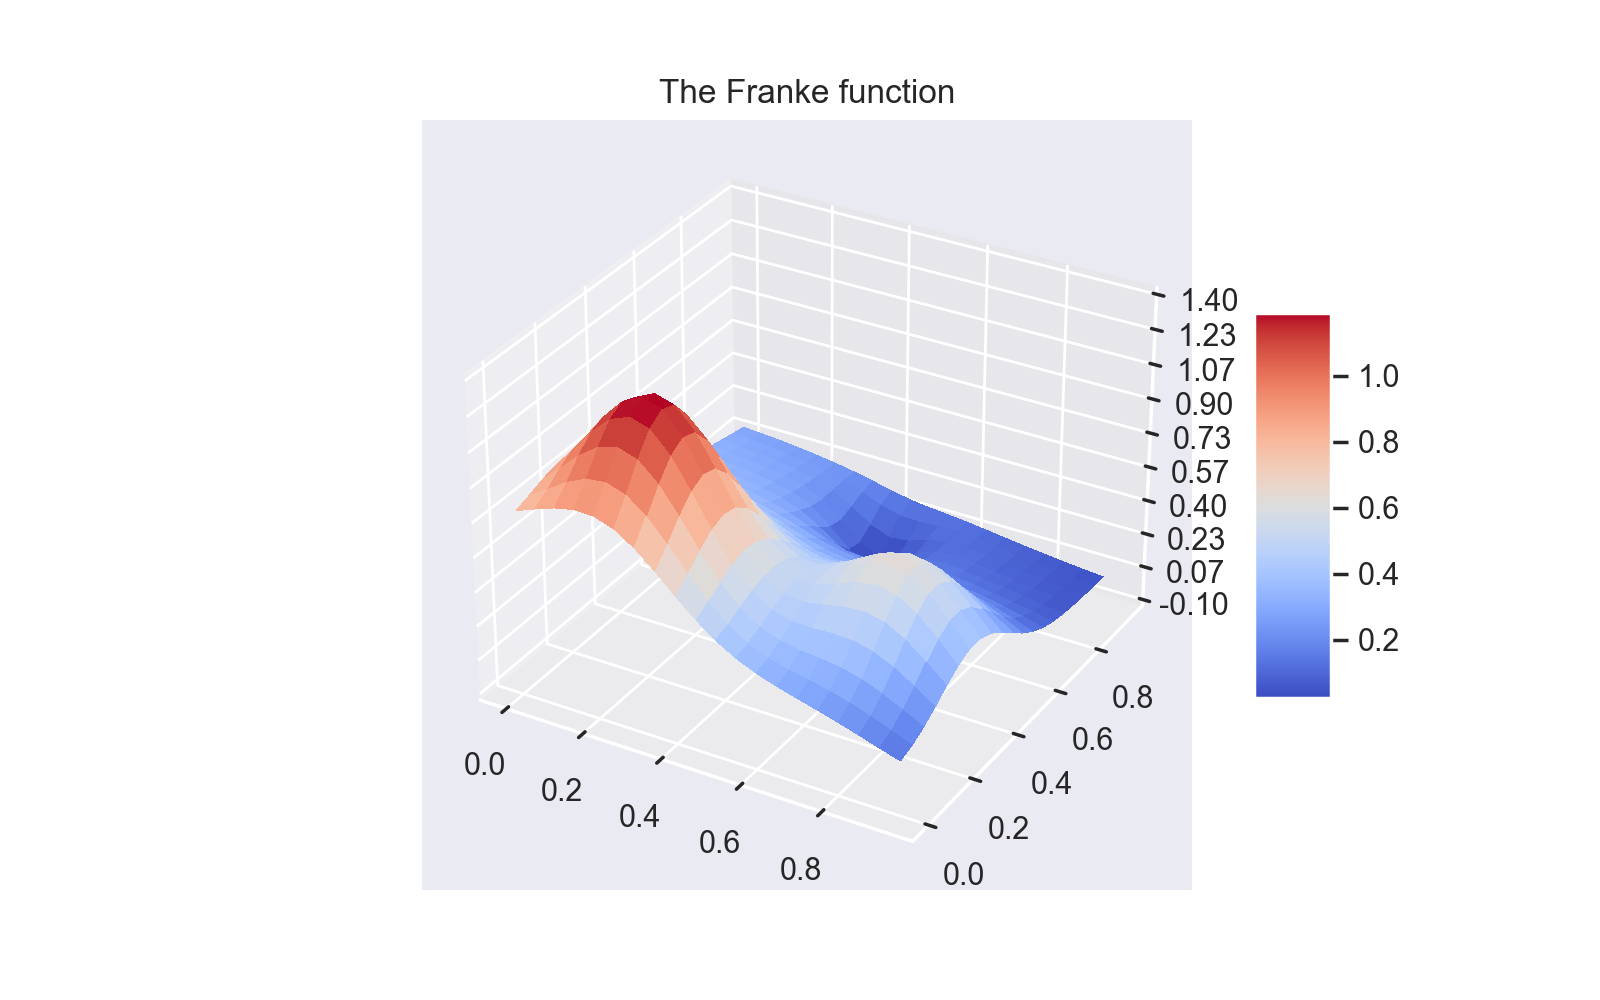
\includegraphics[width=0.5\textwidth]{Figure_1.png}
	\caption{\centering A plot of the Franke function }
	\label{Franke function}
\end{figure}
\noindent This function was fitted with the OLS method, 
and polynomials with varying degrees was used to create the design matrix.
Since the design matrix in this case was noninvertible, singular value 
decomposition was used to create the $\beta$-values needed to create a model
of the dataset. The mean square error and the R2 score was calculated 
for both the testing and training datasets. The result of this analyses is 
shown if figures \eqref{MSE and R2 OLS}, \eqref{MSE and R2 OLS noise} and ...

\noindent Next Ridge and LASSO regression was used on the Franke function,
to see if these methods have a better fit than what was obtained with OLS.
Diffrent values for $\lambda$ was used to obtain the best fit as possible for each
polynomial degree.

\subsection{Cross Validation Methodology}

In the pursuit of assessing the robustness and reliability of Ridge regression models, we employed cross-validation, specifically scrutinizing the impact of varying regularization parameters, denoted as \(\lambda\). The function \texttt{k\_fold}, was developed to execute the k-fold cross-validation technique, accepting the dataset and an integer \(k\) as arguments, and subsequently partitioning the data into \(k\) randomized subsets (folds). It returns \(k\) pairs of training and test indices, each representing a distinct division of the data, enabling model evaluation across varied data scenarios.
For each \(\lambda\) value in a logarithmically spaced array of \(\lambda\) values, denoted \texttt{lambdas}, the Ridge regression model was trained and validated \(k\) times - once per fold. Specifically, for every tuple \((\text{train\_indices}, \text{test\_indices})\) produced by \texttt{k\_fold(data, k)}, the data was divided into training and test sets \((x_{\text{train}}, y_{\text{train}}, x_{\text{test}}, y_{\text{test}})\).
Subsequently, the \texttt{design\_matrix} function generated polynomial feature matrices \(X_{\text{train}}\) and \(X_{\text{test}}\) from the \(x\) and \(y\) values, using a specified polynomial degree. The Ridge model, instantiated with the current \(\lambda\), was then fitted with \(X_{\text{train}}\) and \(y_{\text{train}}\), and predictions \(y_{\text{pred}}\) were made using \(X_{\text{test}}\). The Mean Squared Error (MSE) between the predictions and actual test values \(y_{\text{test}}\) was computed and stored in a scores array.
The MSE values were averaged per \(\lambda\), providing an unbiased performance metric, and facilitating the analysis and visualization of how distinct regularization parameters influenced model performance.



\section{Results}
\thispagestyle{plain}
\subsection{Result for Franke function}
\noindent Our initial step involved the application of OLS to the Franke function without noise
This analysis was conducted without employing any resampling techniques, 
and our dataset conisted of 100 data points. The results for the MSE and R2 score is shown in 
figure \eqref{MSE and R2 OLS}

\begin{figure}[h]
	\centering
	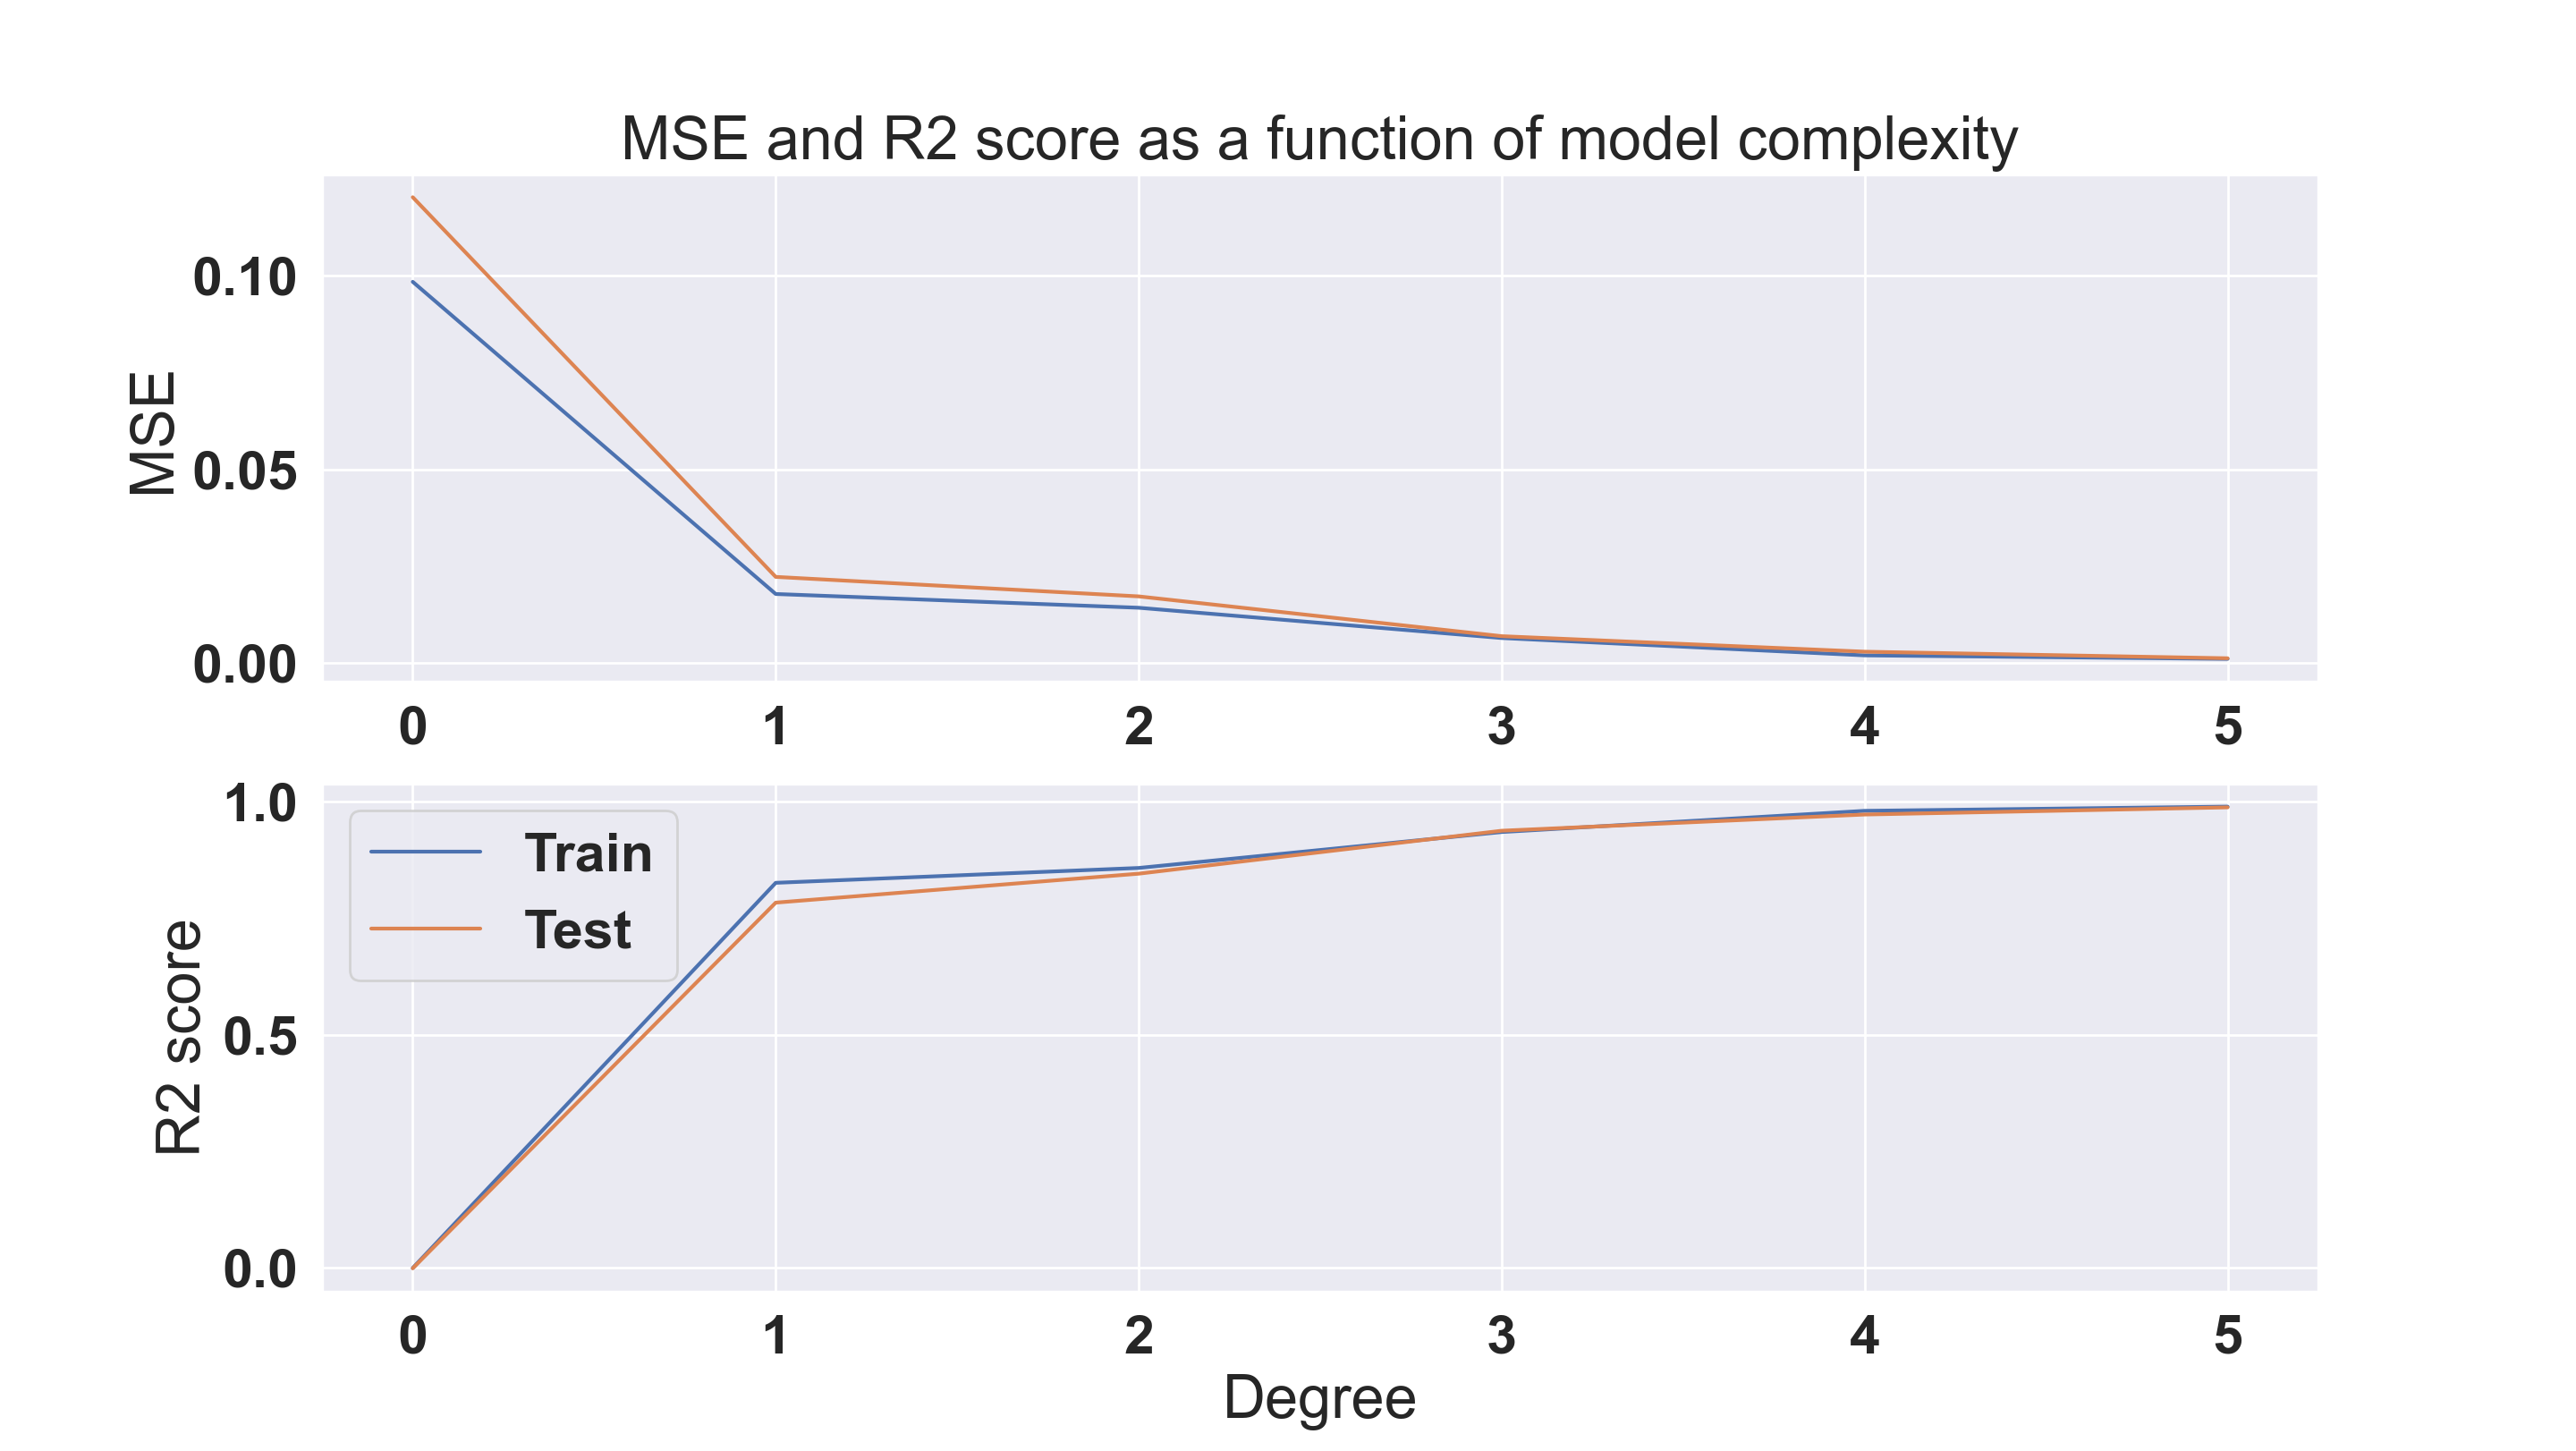
\includegraphics[width=0.5\textwidth]{Figure_3.png}
	\caption{Plot showing the MSE and R2 score for the franke function without noise. The regression method used was OLS}
	\label{MSE and R2 OLS}
\end{figure}
\noindent The next step was to include noise given by the normal distribution $\mathcal{N}(0,0.1)$. Figure \eqref{MSE and R2 OLS noise} shows
how the MSE and R2 score changes when noise is includet in to the data set.
\begin{figure}[h]
	\centering
	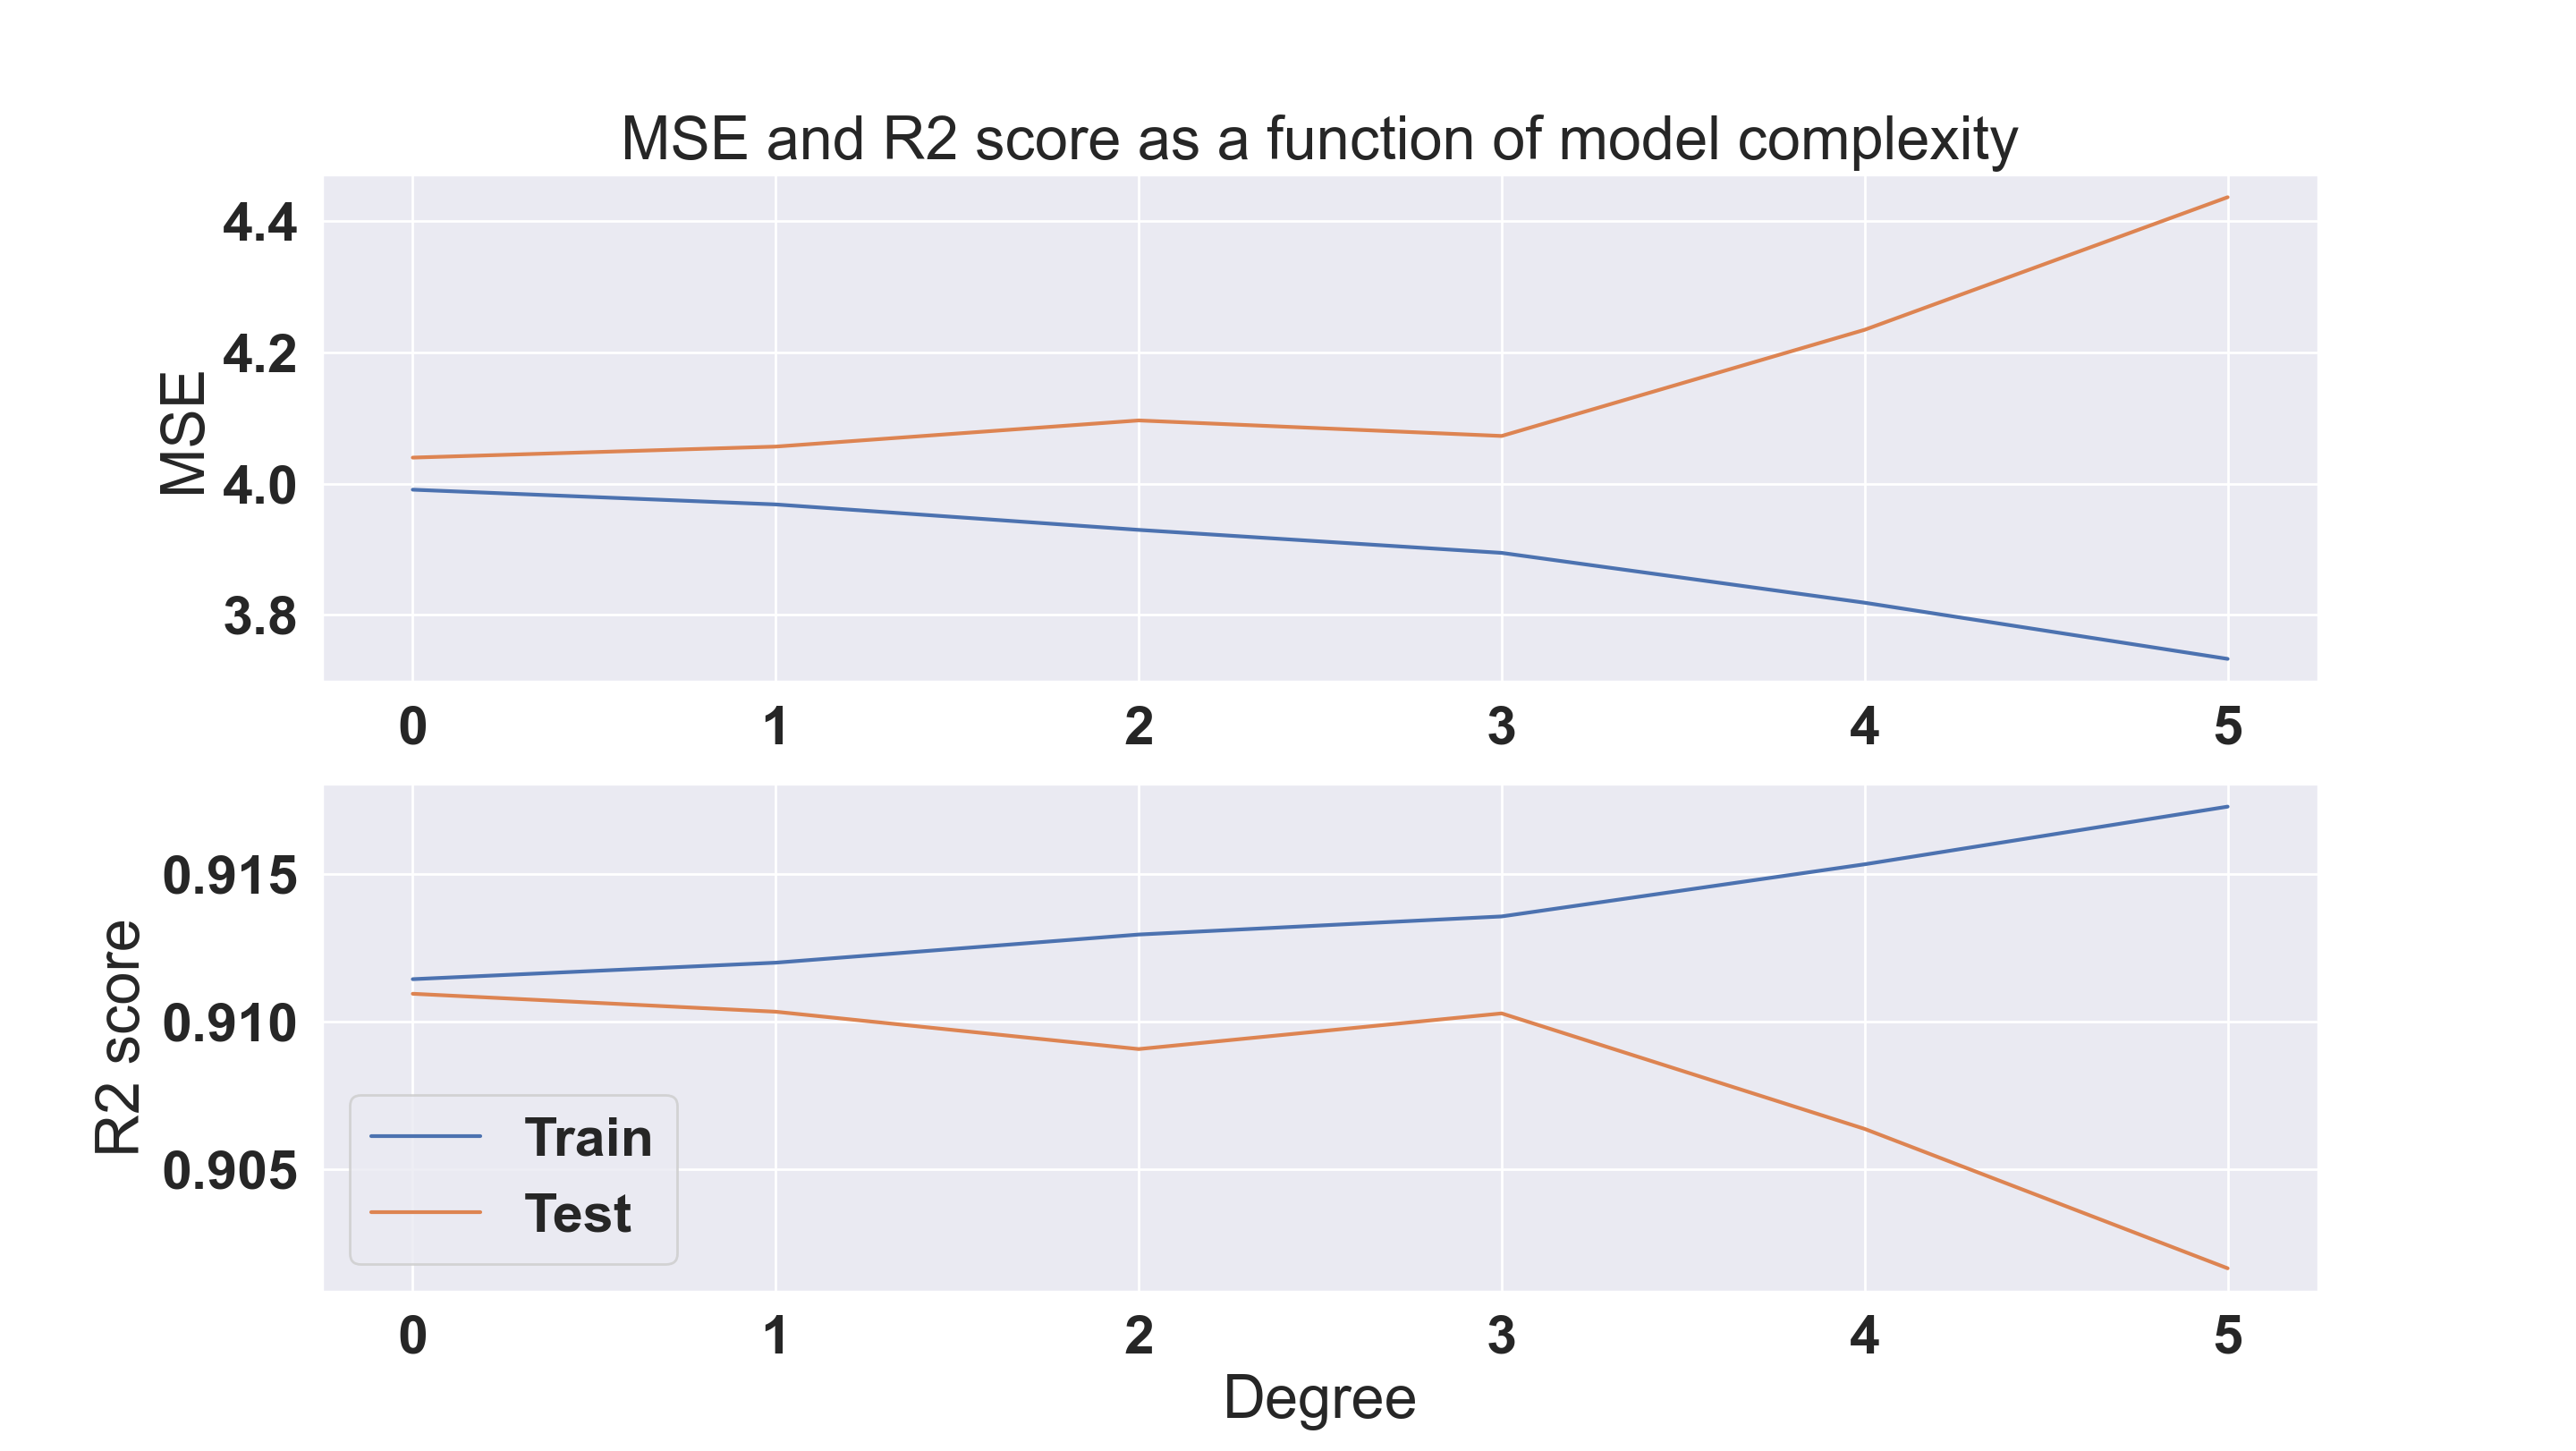
\includegraphics[width=0.5\textwidth]{Figure_4.png}
	\caption{Plot showing the MSE and R2 score for the franke function with noise $\mathcal{N}(0,0.1)$. The regression method used was OLS}
	\label{MSE and R2 OLS noise}
\end{figure}

\begin{figure}[h]
	\centering
	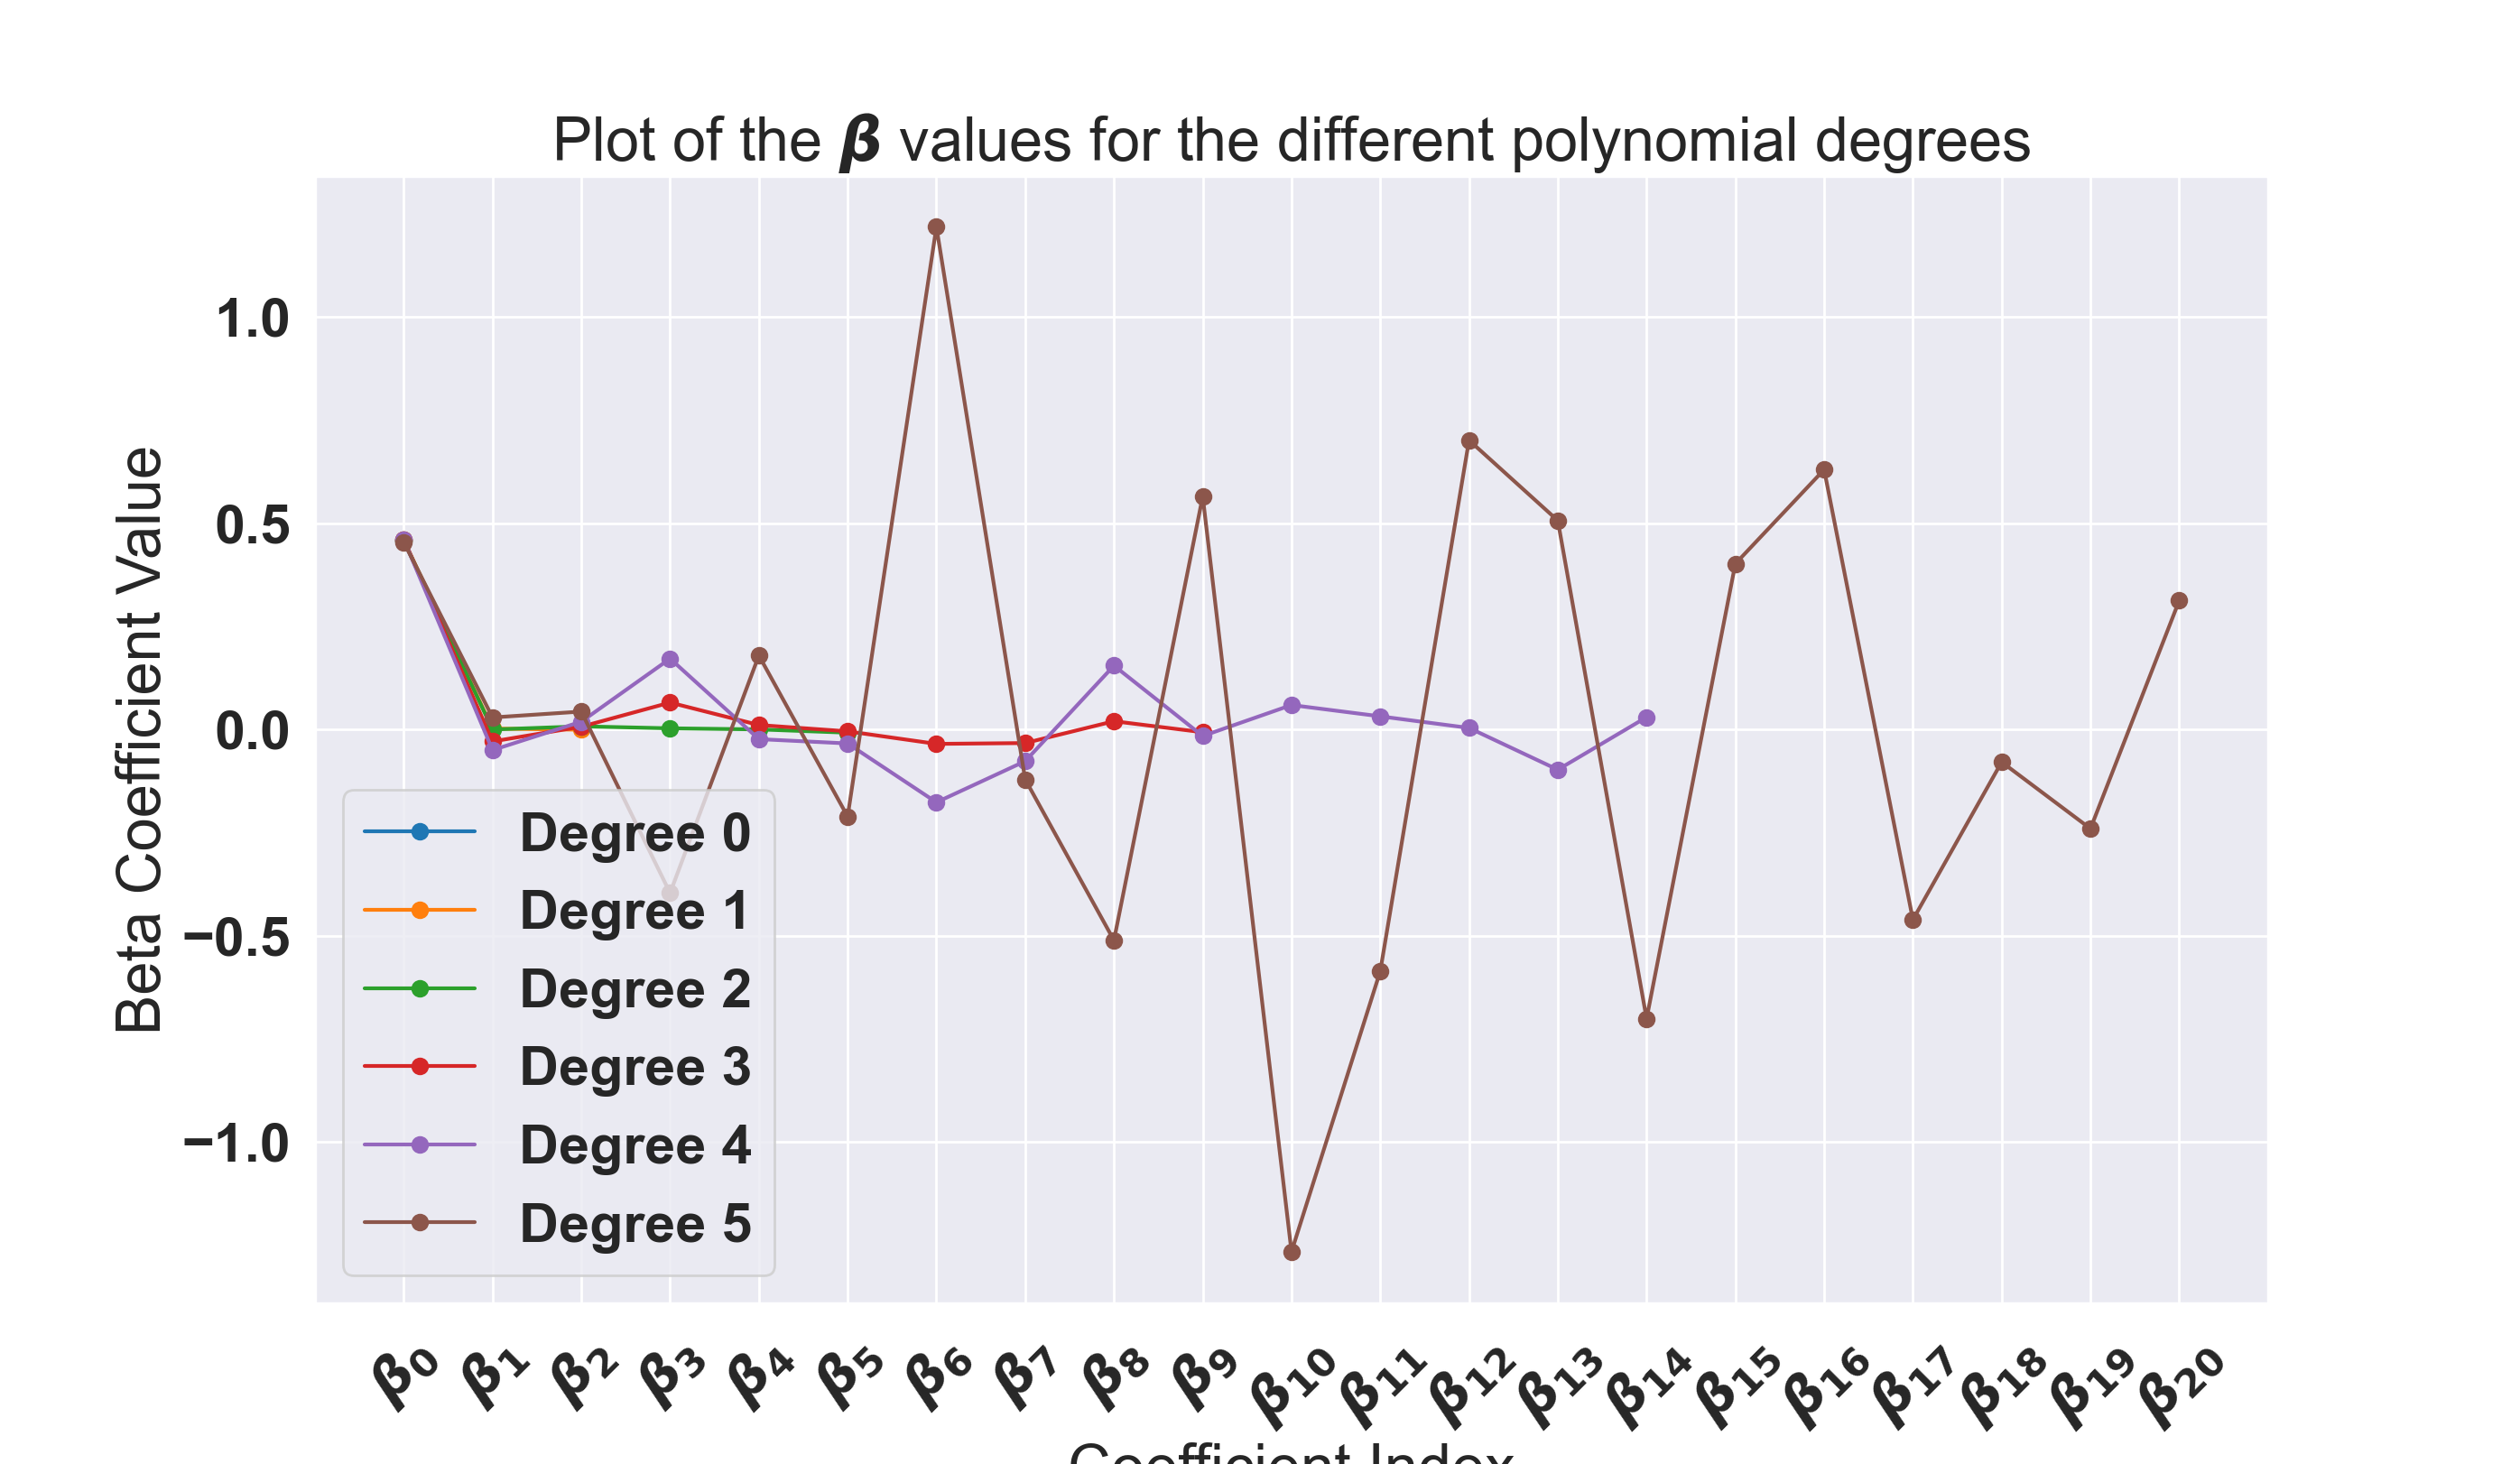
\includegraphics[width=0.5\textwidth]{Figure_12.png}
	\caption{}
	\label{beta OLS}
\end{figure}



\noindent For Ridge Regression on the franke function have we plotted a heatmap to show 
how the MSE changes with diffrent $\lambda$ values and complexities. A plot of
the heatmap for the training data is shown in figure \eqref{heatmap training ridge}
, and the heatmap for the test data is shown in figure \eqref{heatmap test ridge}.
\begin{figure}[h]
	\centering
	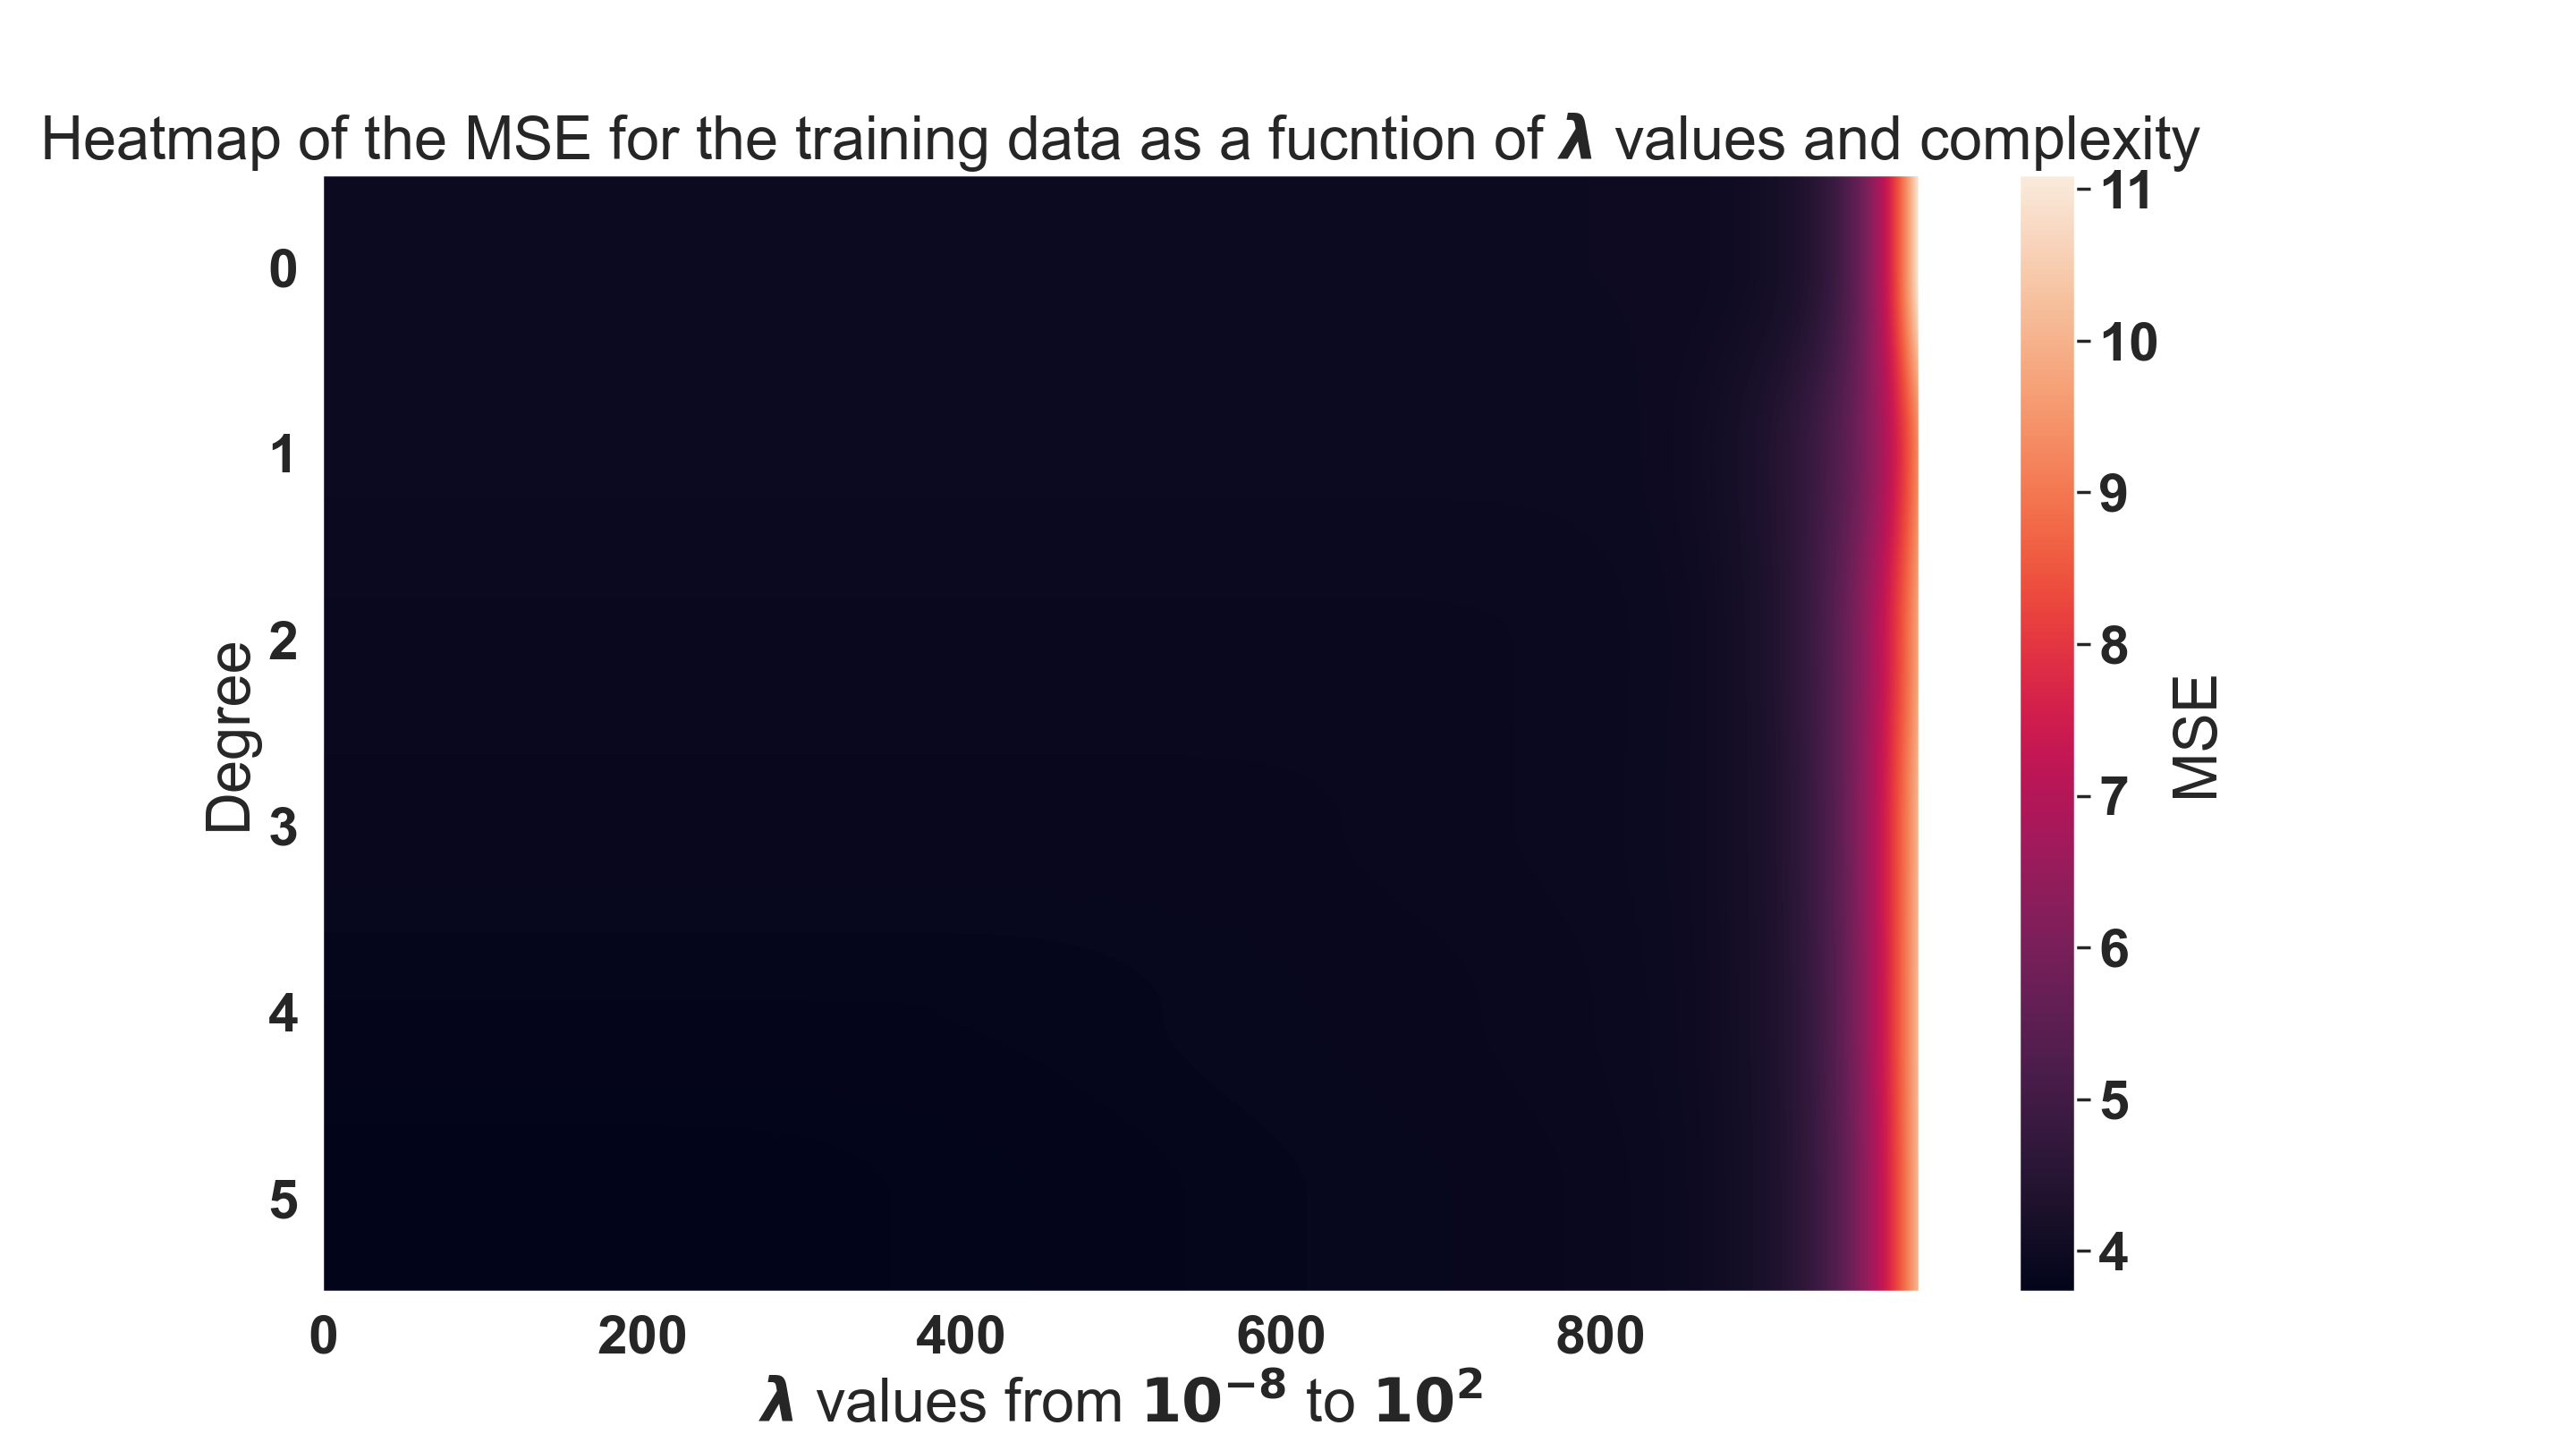
\includegraphics[width=0.5\textwidth]{Figure_8.png}
	\caption{A heatmap of the MSE for the training data, for different $\lambda$ values and complexities. The $\lambda$ values goes from $10^{-8}$ to $10^{2}$ }
	\label{heatmap training ridge}
\end{figure}
\begin{figure}[h]
	\centering
	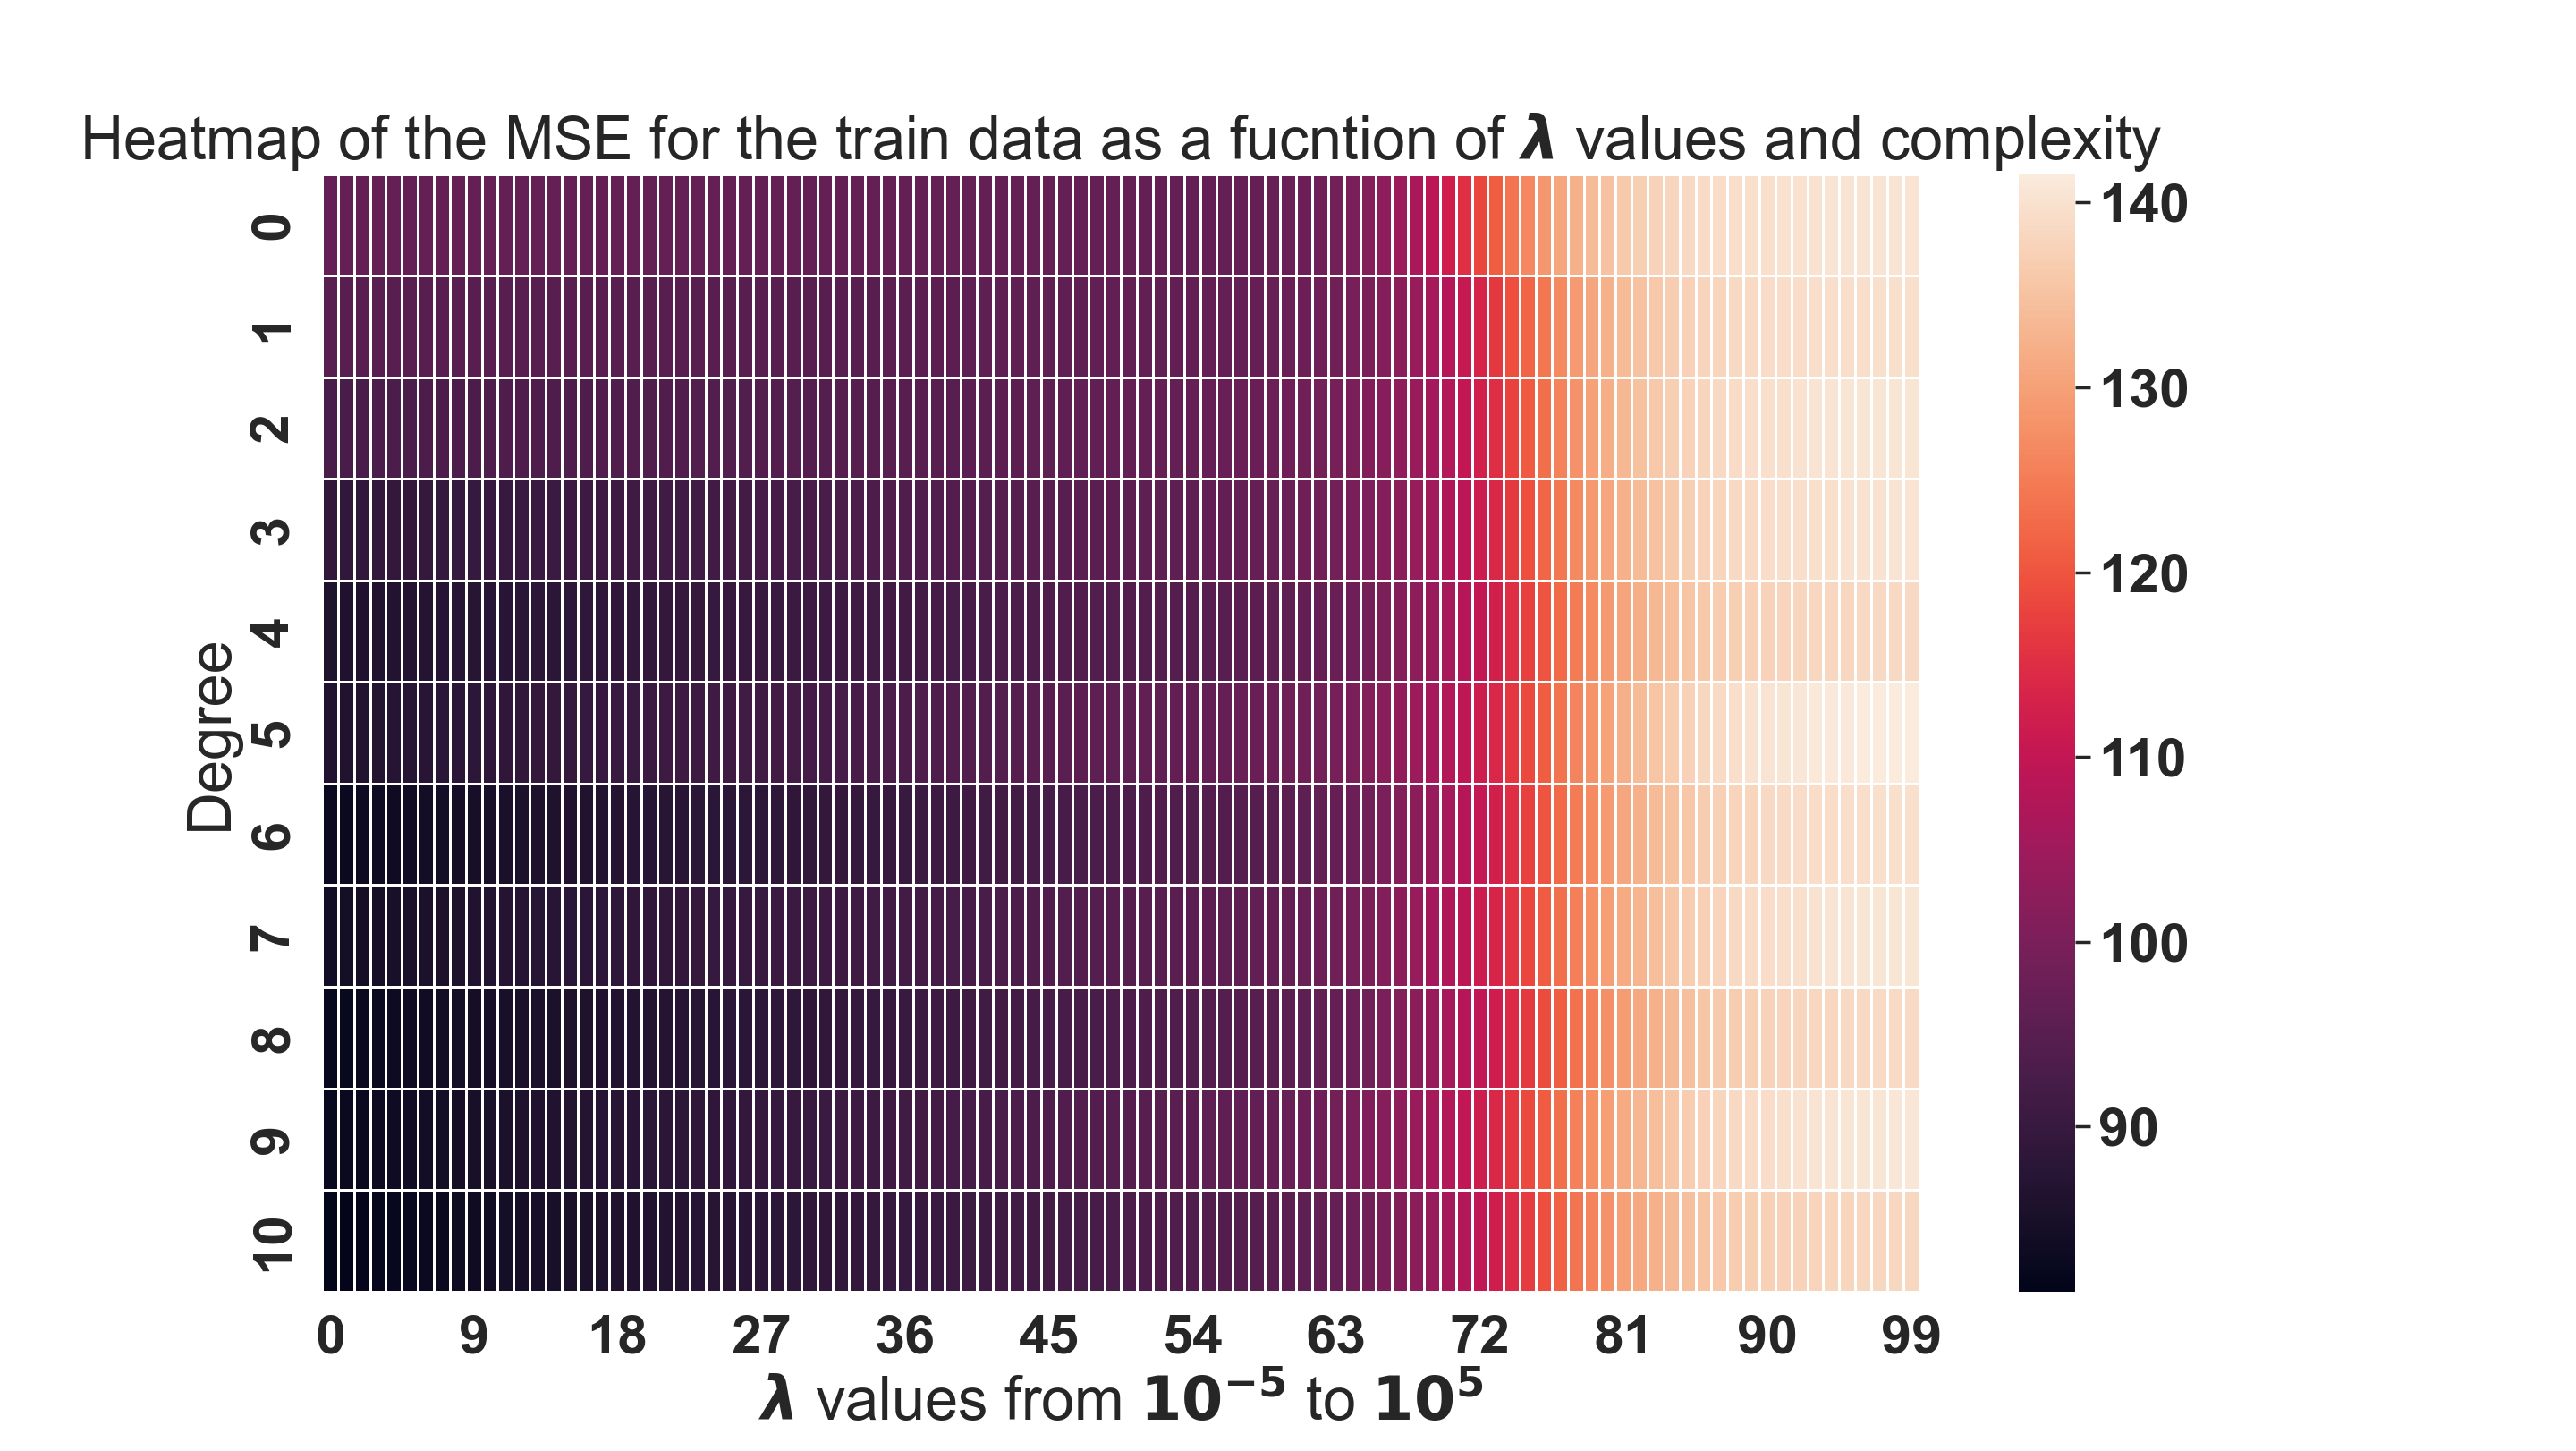
\includegraphics[width=0.5\textwidth]{Figure_7.png}
	\caption{A heatmap of the MSE for the testing data, for different $\lambda$ values and complexities. The $\lambda$ values goes from $10^{-5}$ to $10^{5}$}
	\label{heatmap test ridge}
\end{figure}
Lastly for Ridge regression we see what happens when $\lambda$ is put to zero.




\begin{figure}[h]
	\centering
	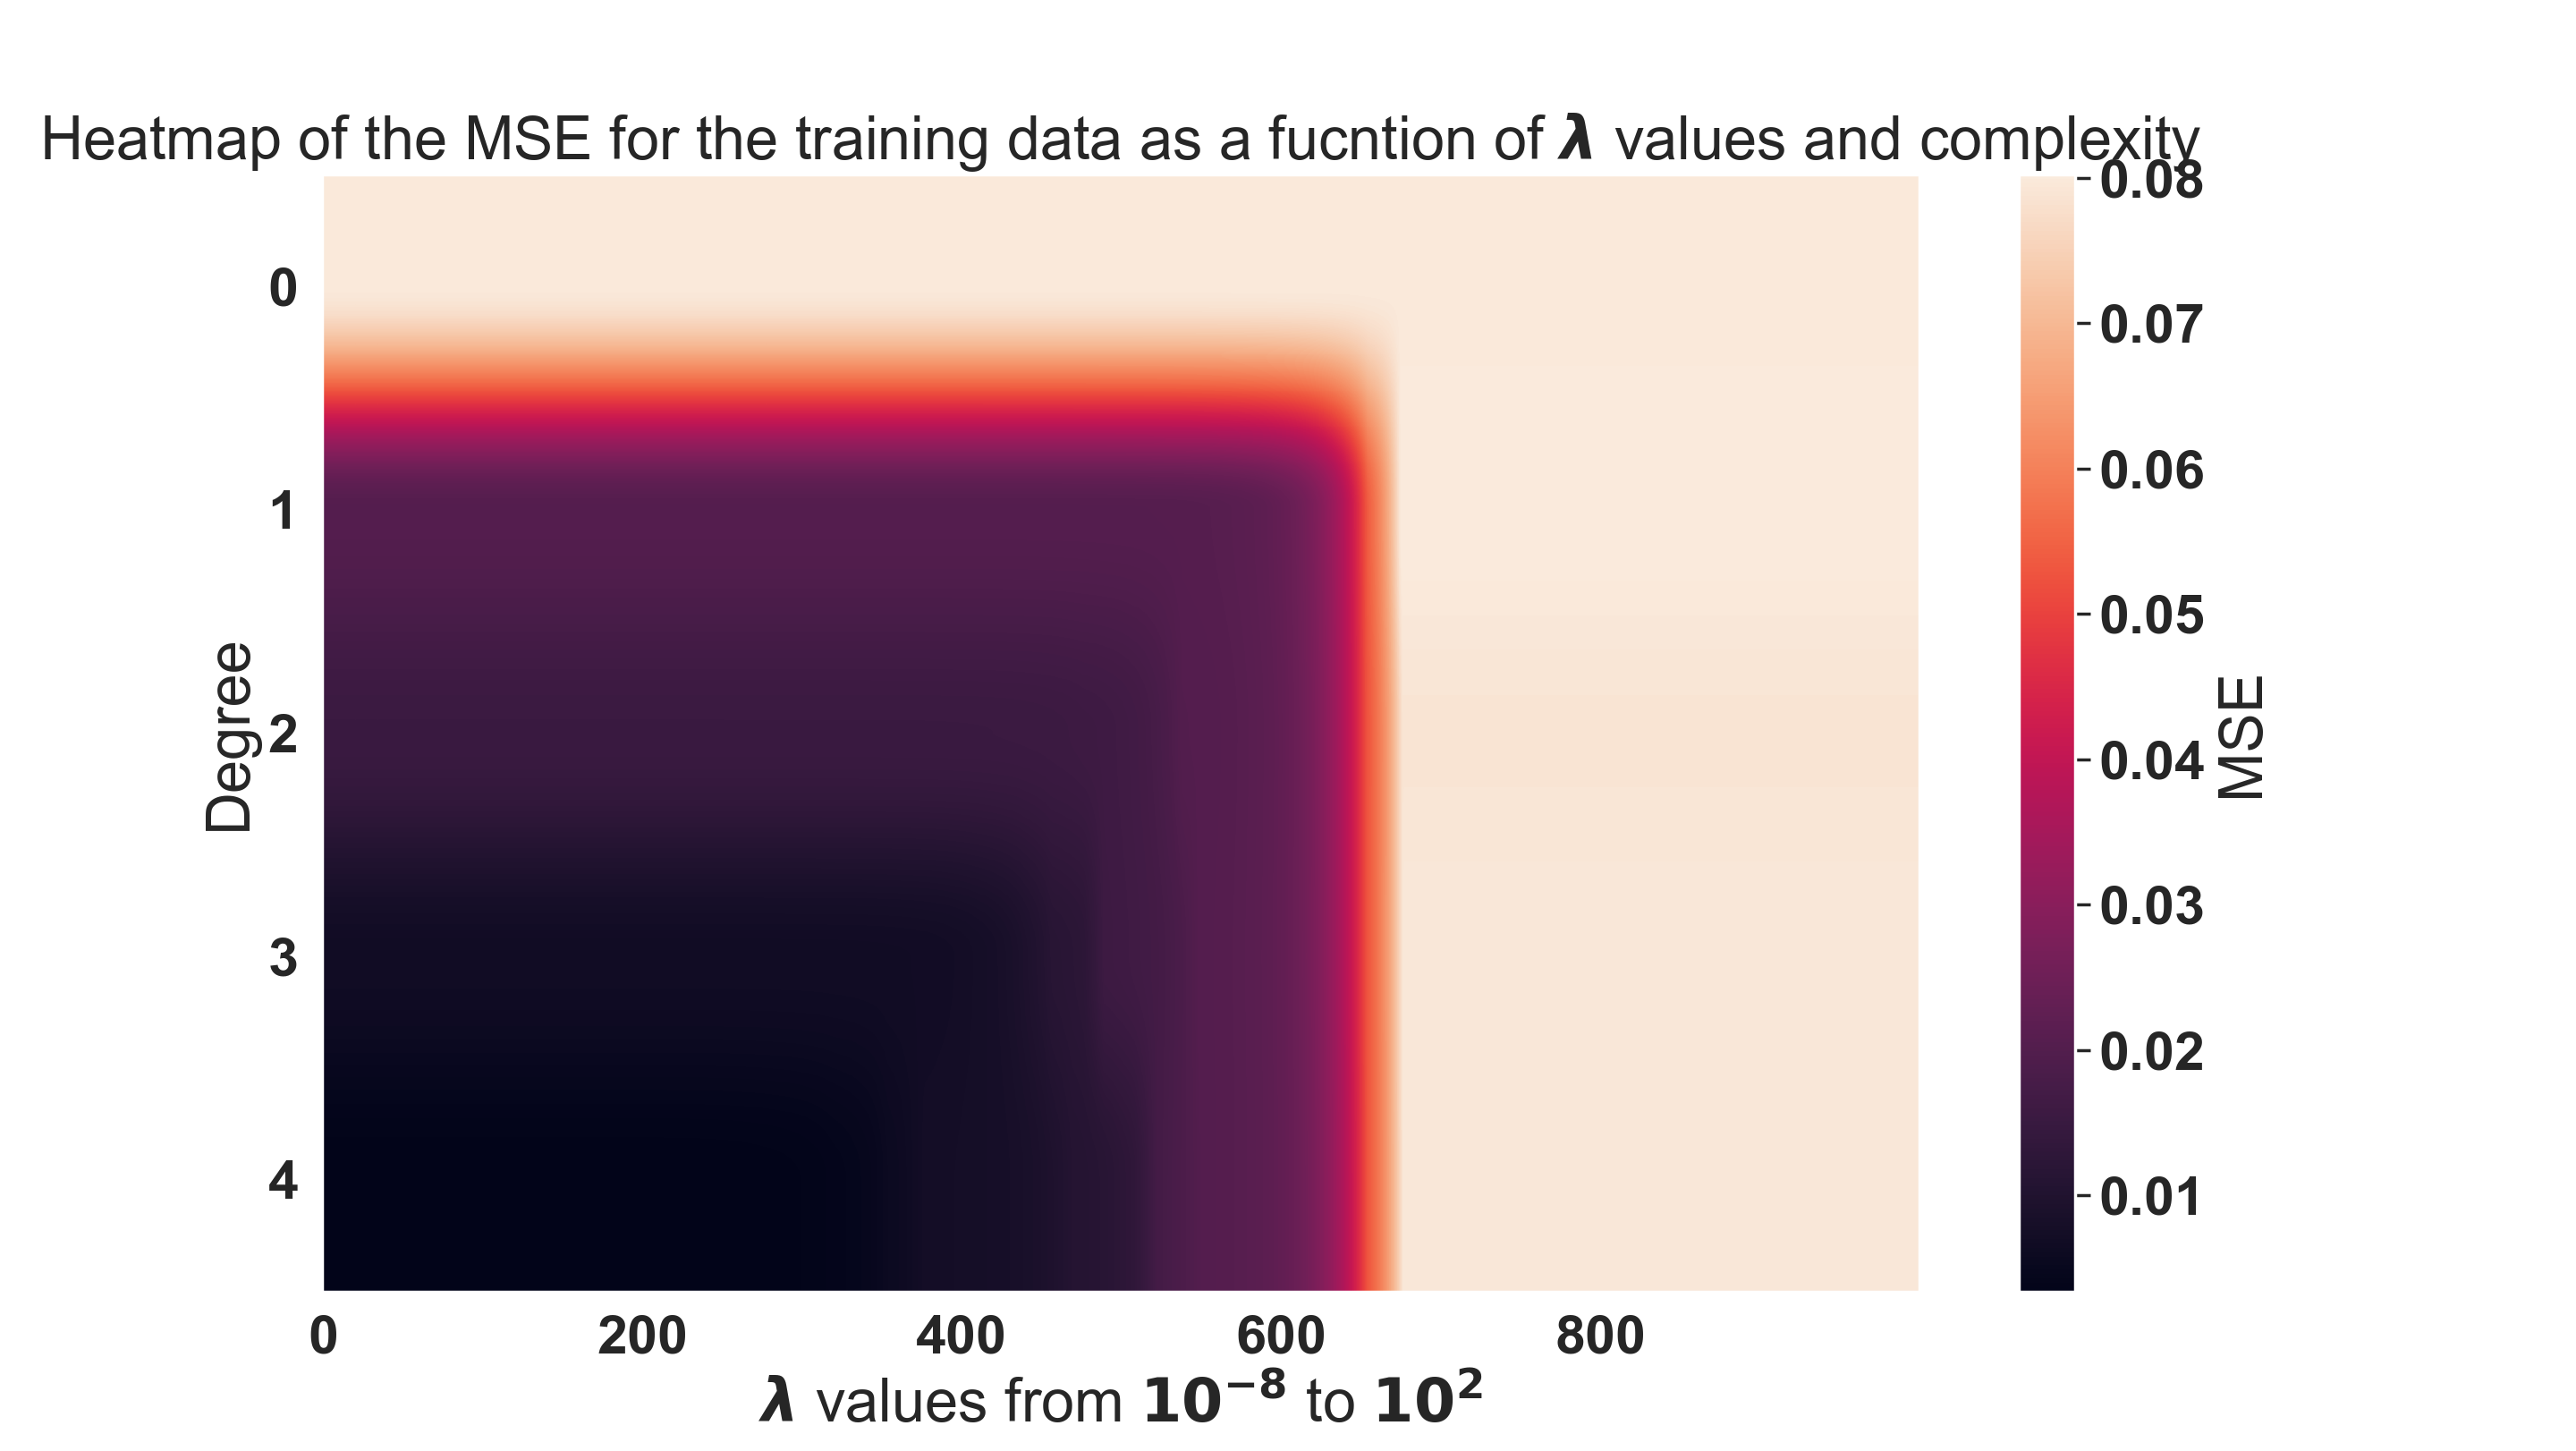
\includegraphics[width=0.5\textwidth]{Figure_9.png}
	\caption{A heatmap of the MSE for the training data, for different $\lambda$ values and complexities. The $\lambda$ values goes from $10^{-8}$ to $10^{2}$ }
	\label{heatmap training LASSO}
\end{figure}
\begin{figure}[h]
	\centering
	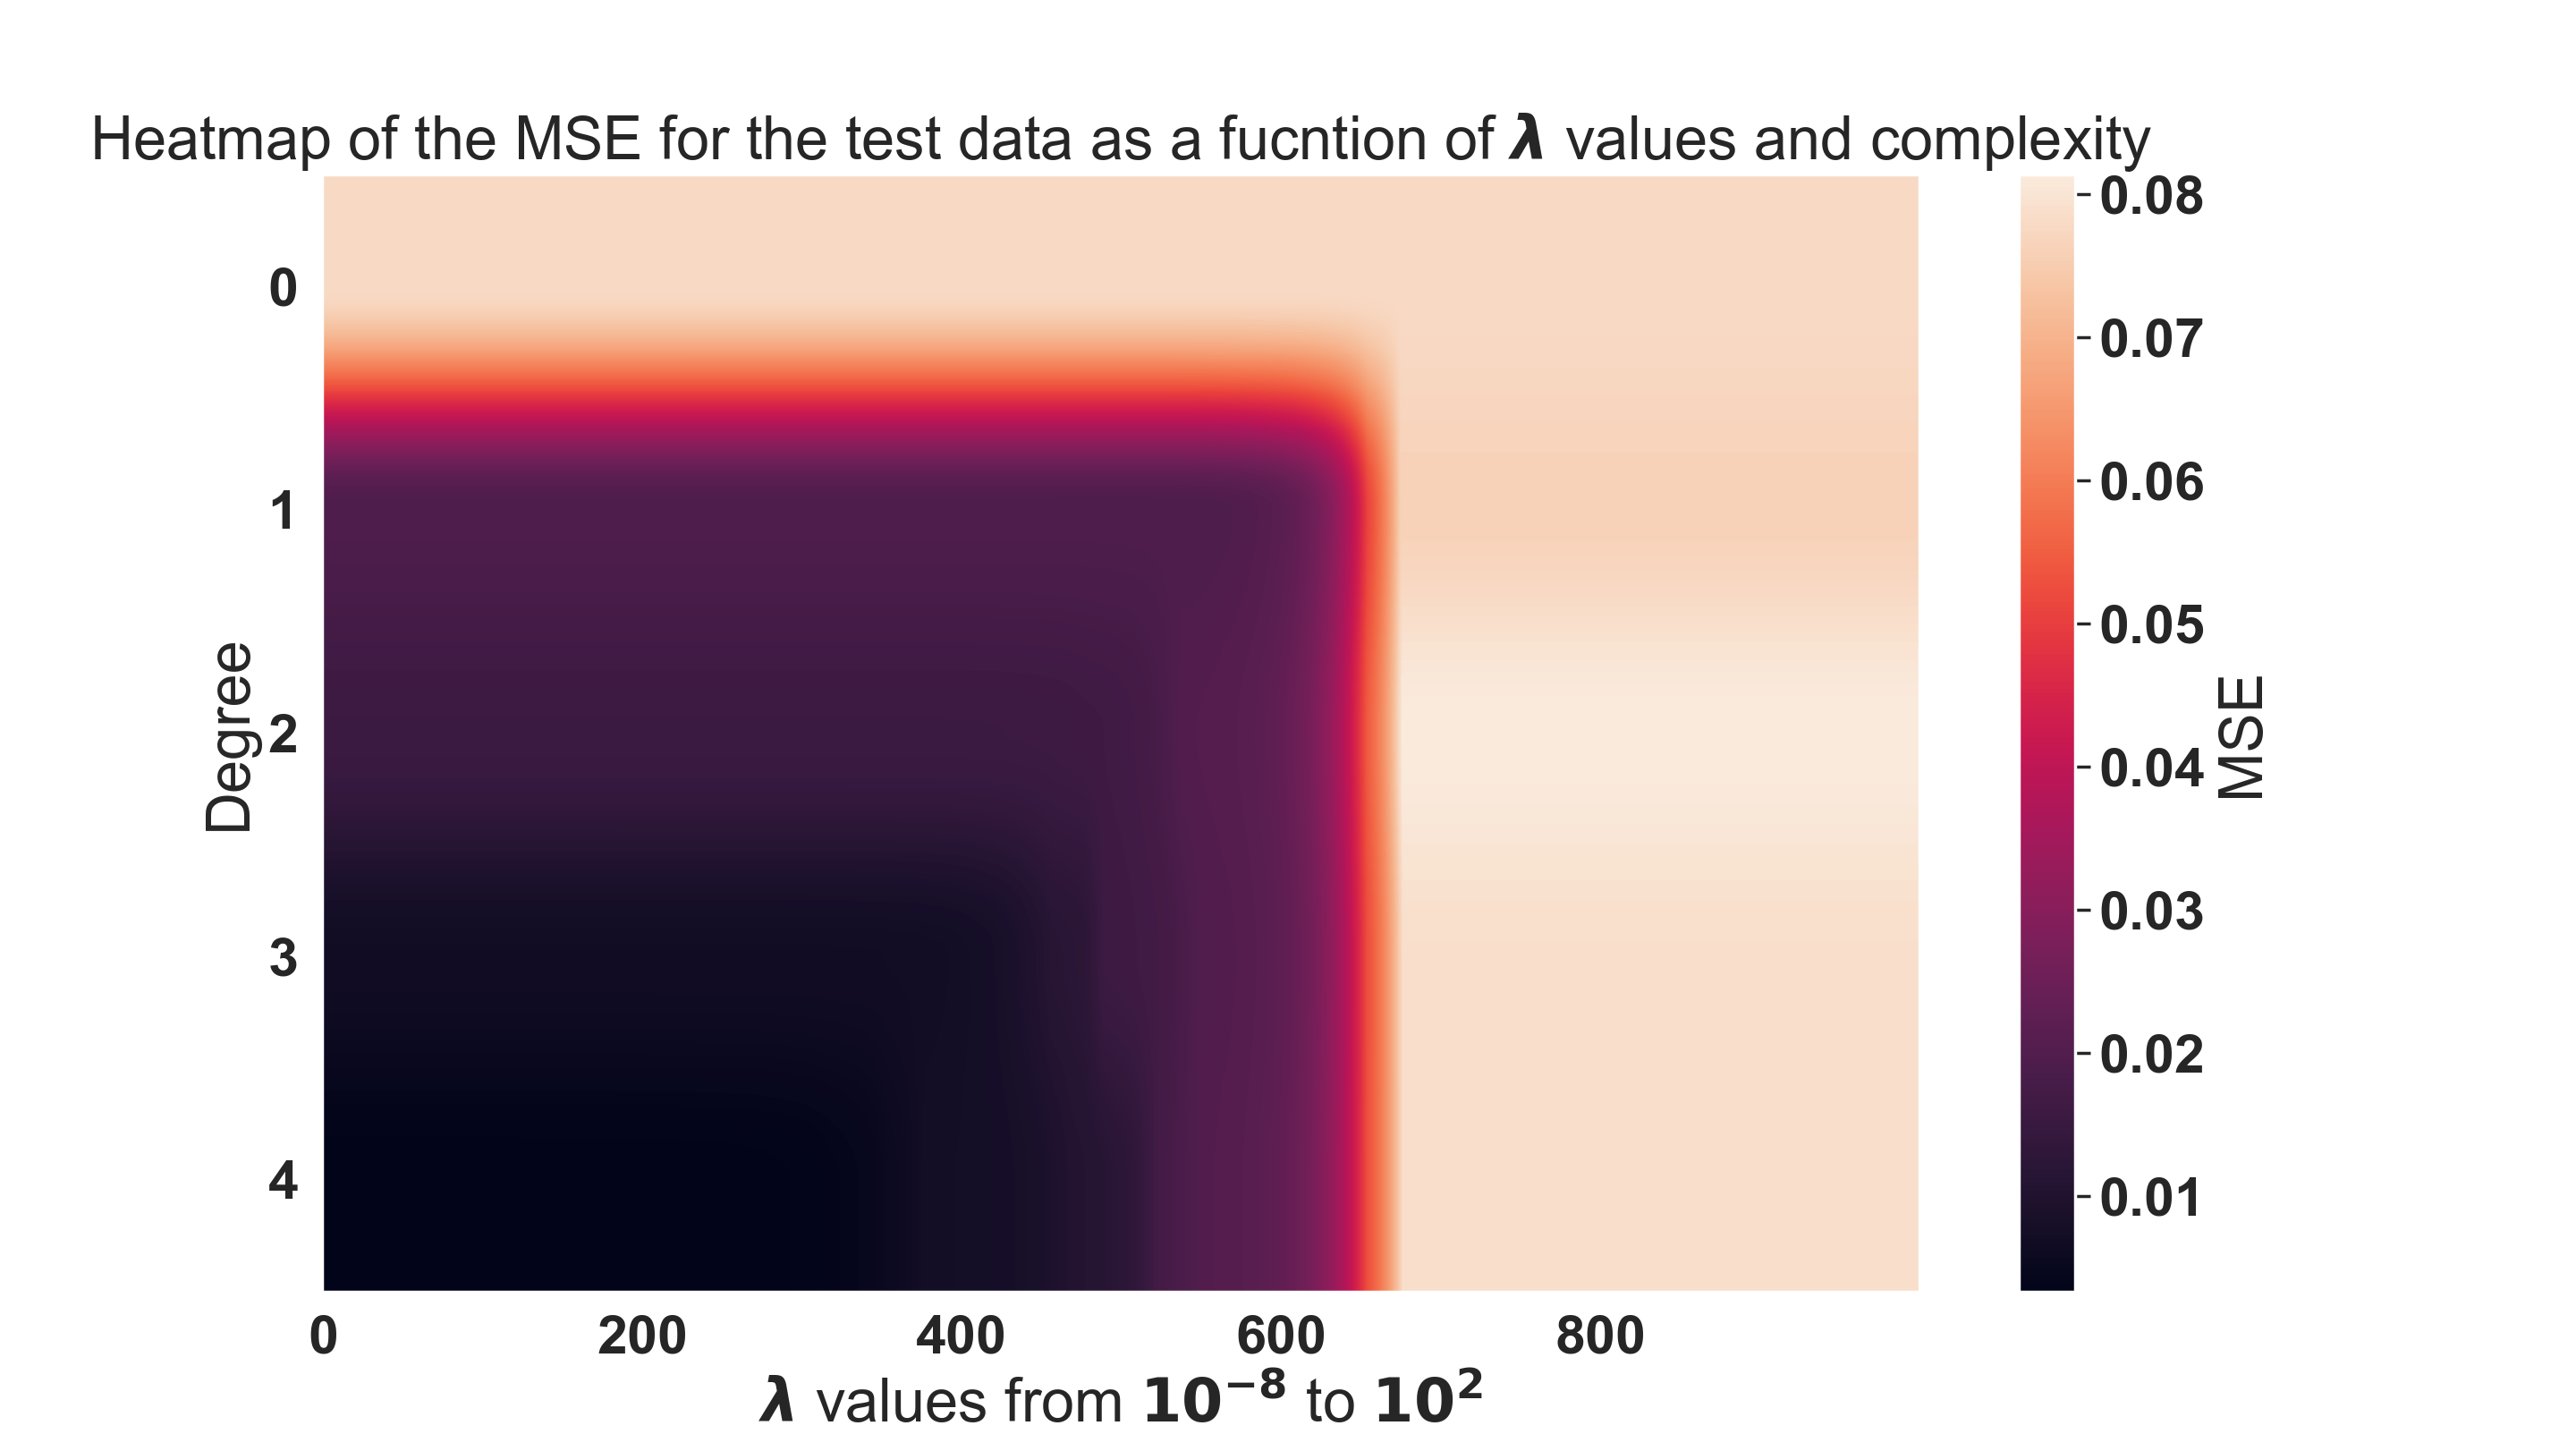
\includegraphics[width=0.5\textwidth]{Figure_10.png}
	\caption{A heatmap of the MSE for the testing data, for different $\lambda$ values and complexities. The $\lambda$ values goes from $10^{-5}$ to $10^{5}$}
	\label{heatmap test LASSO}
\end{figure}




\begin{figure*}[h]
	\centering
	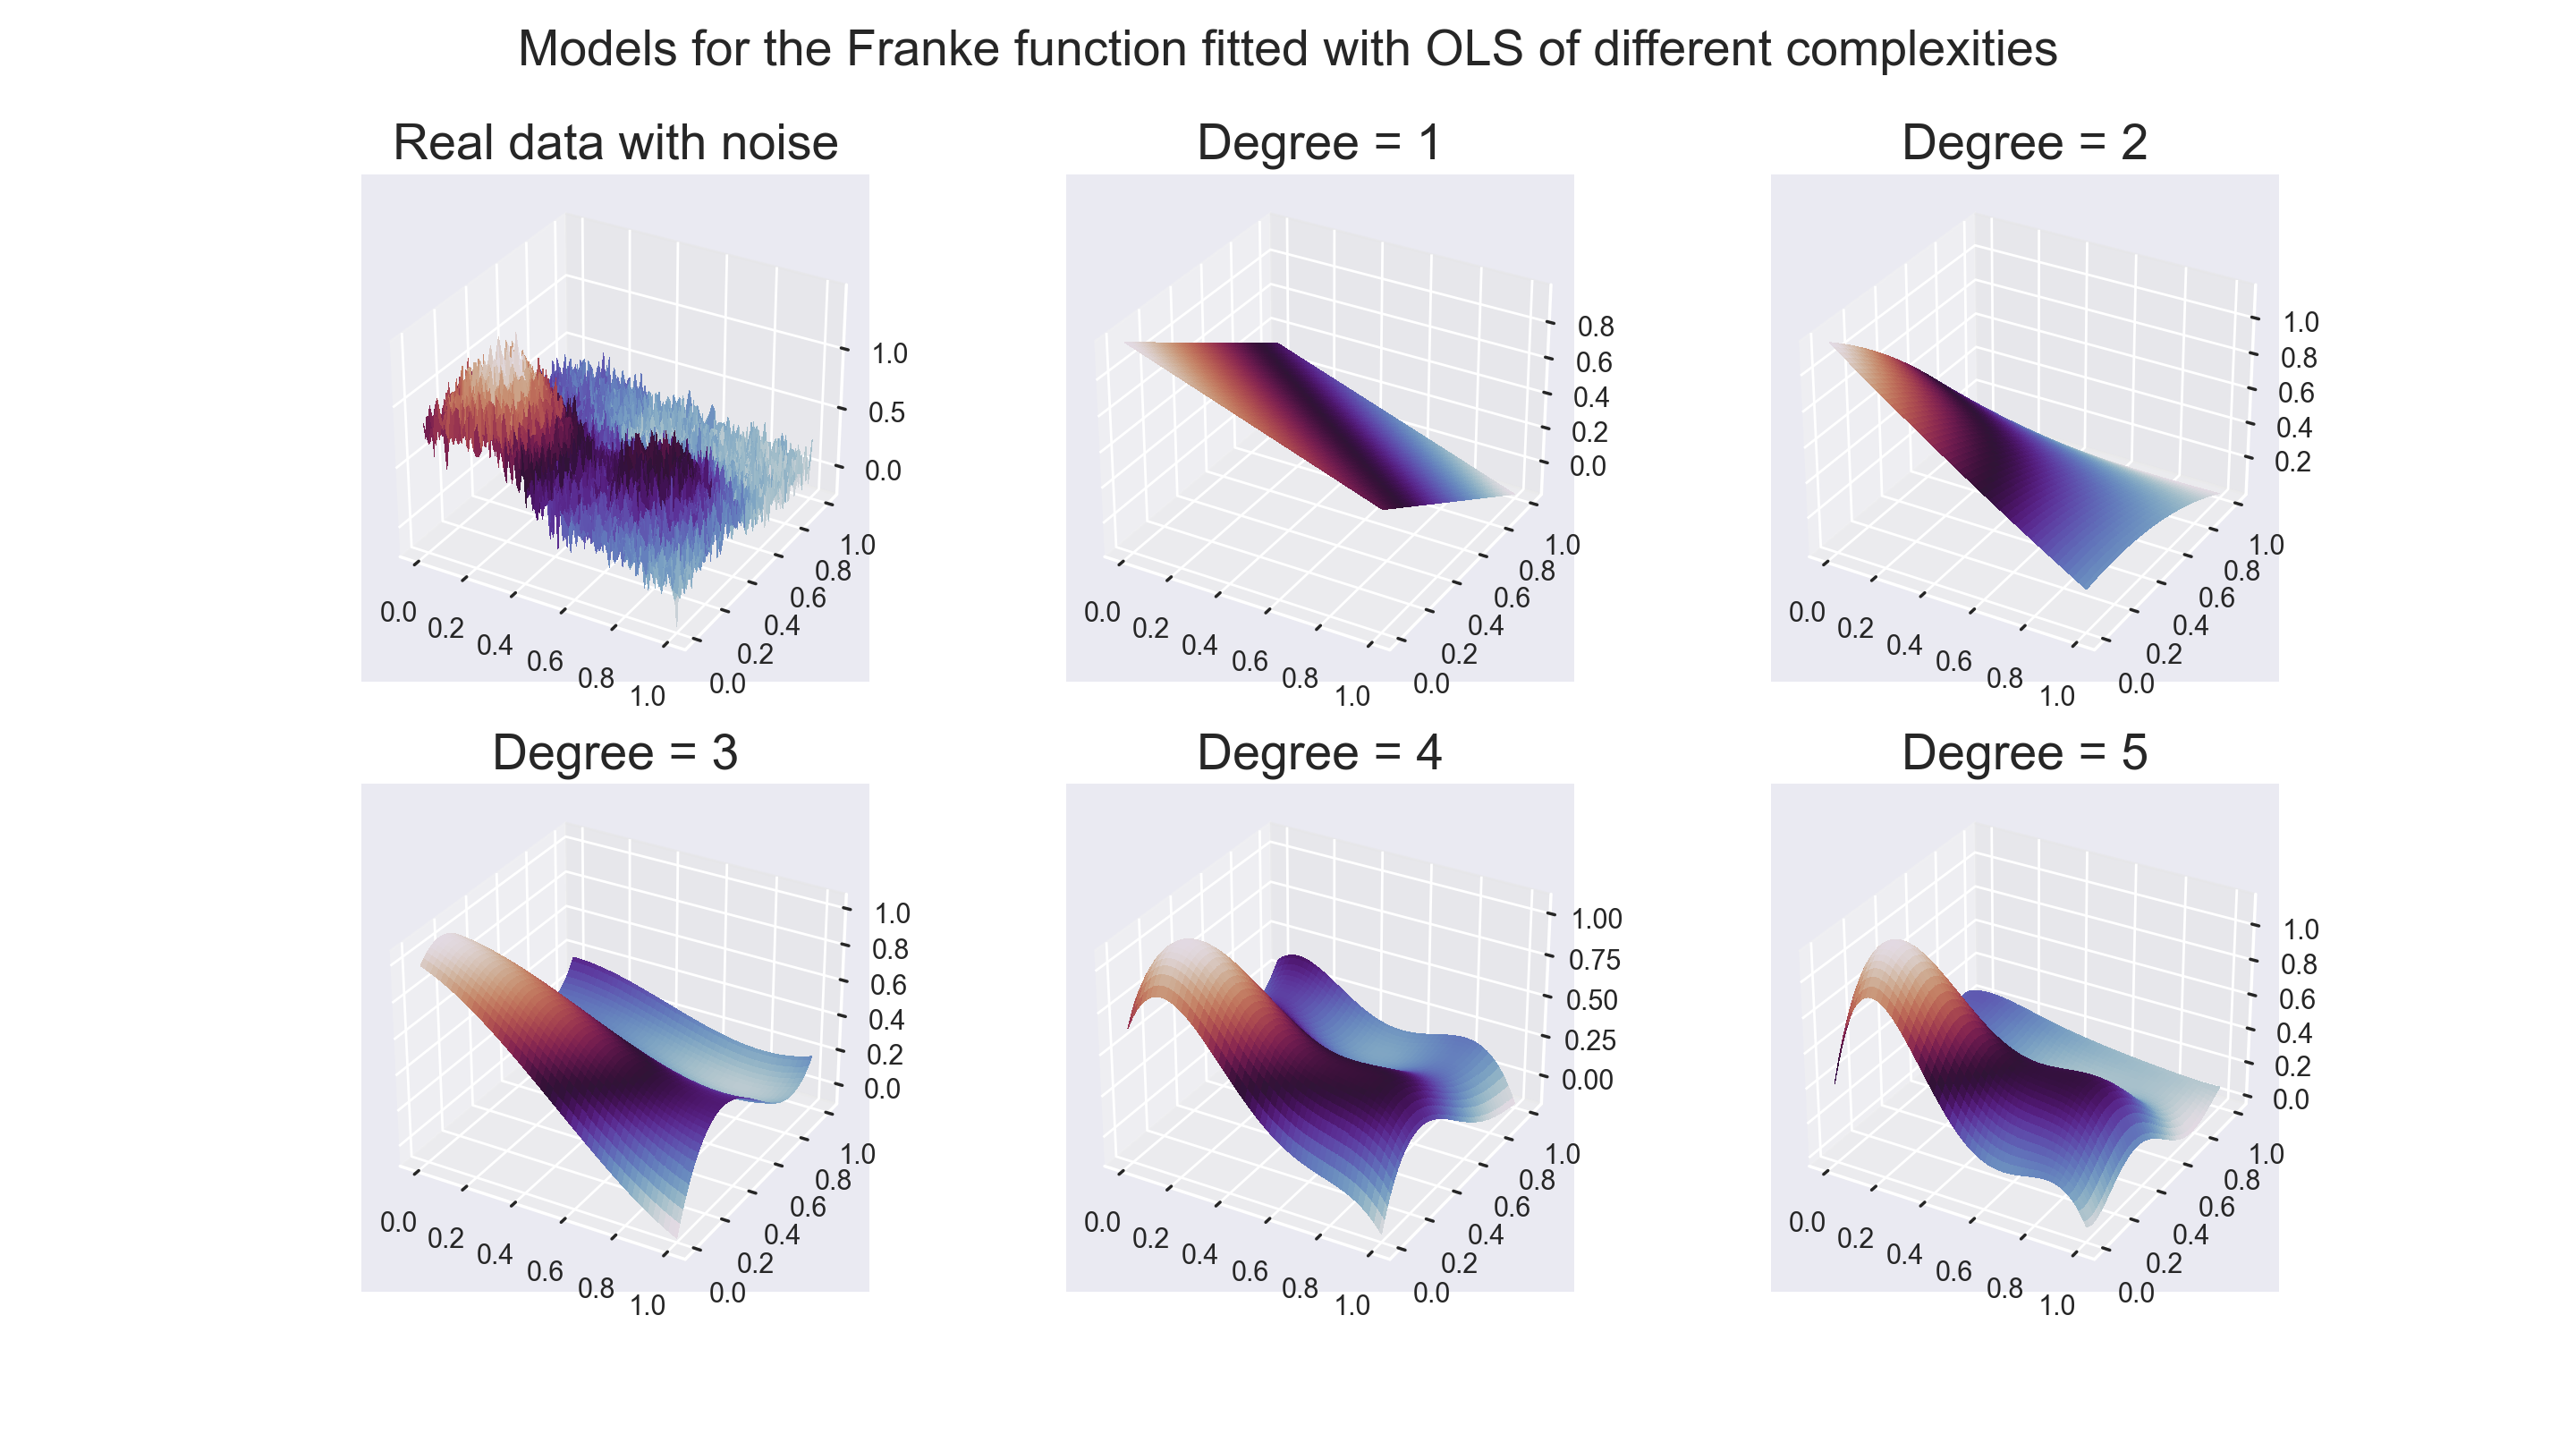
\includegraphics[width=\textwidth]{Figure_2.png}
	\caption{A plot showing how model with different complexities fit the franke function when OLS regession has been used.}
	\label{OLS figure}
\end{figure*}


\begin{figure*}[h]
	\centering
	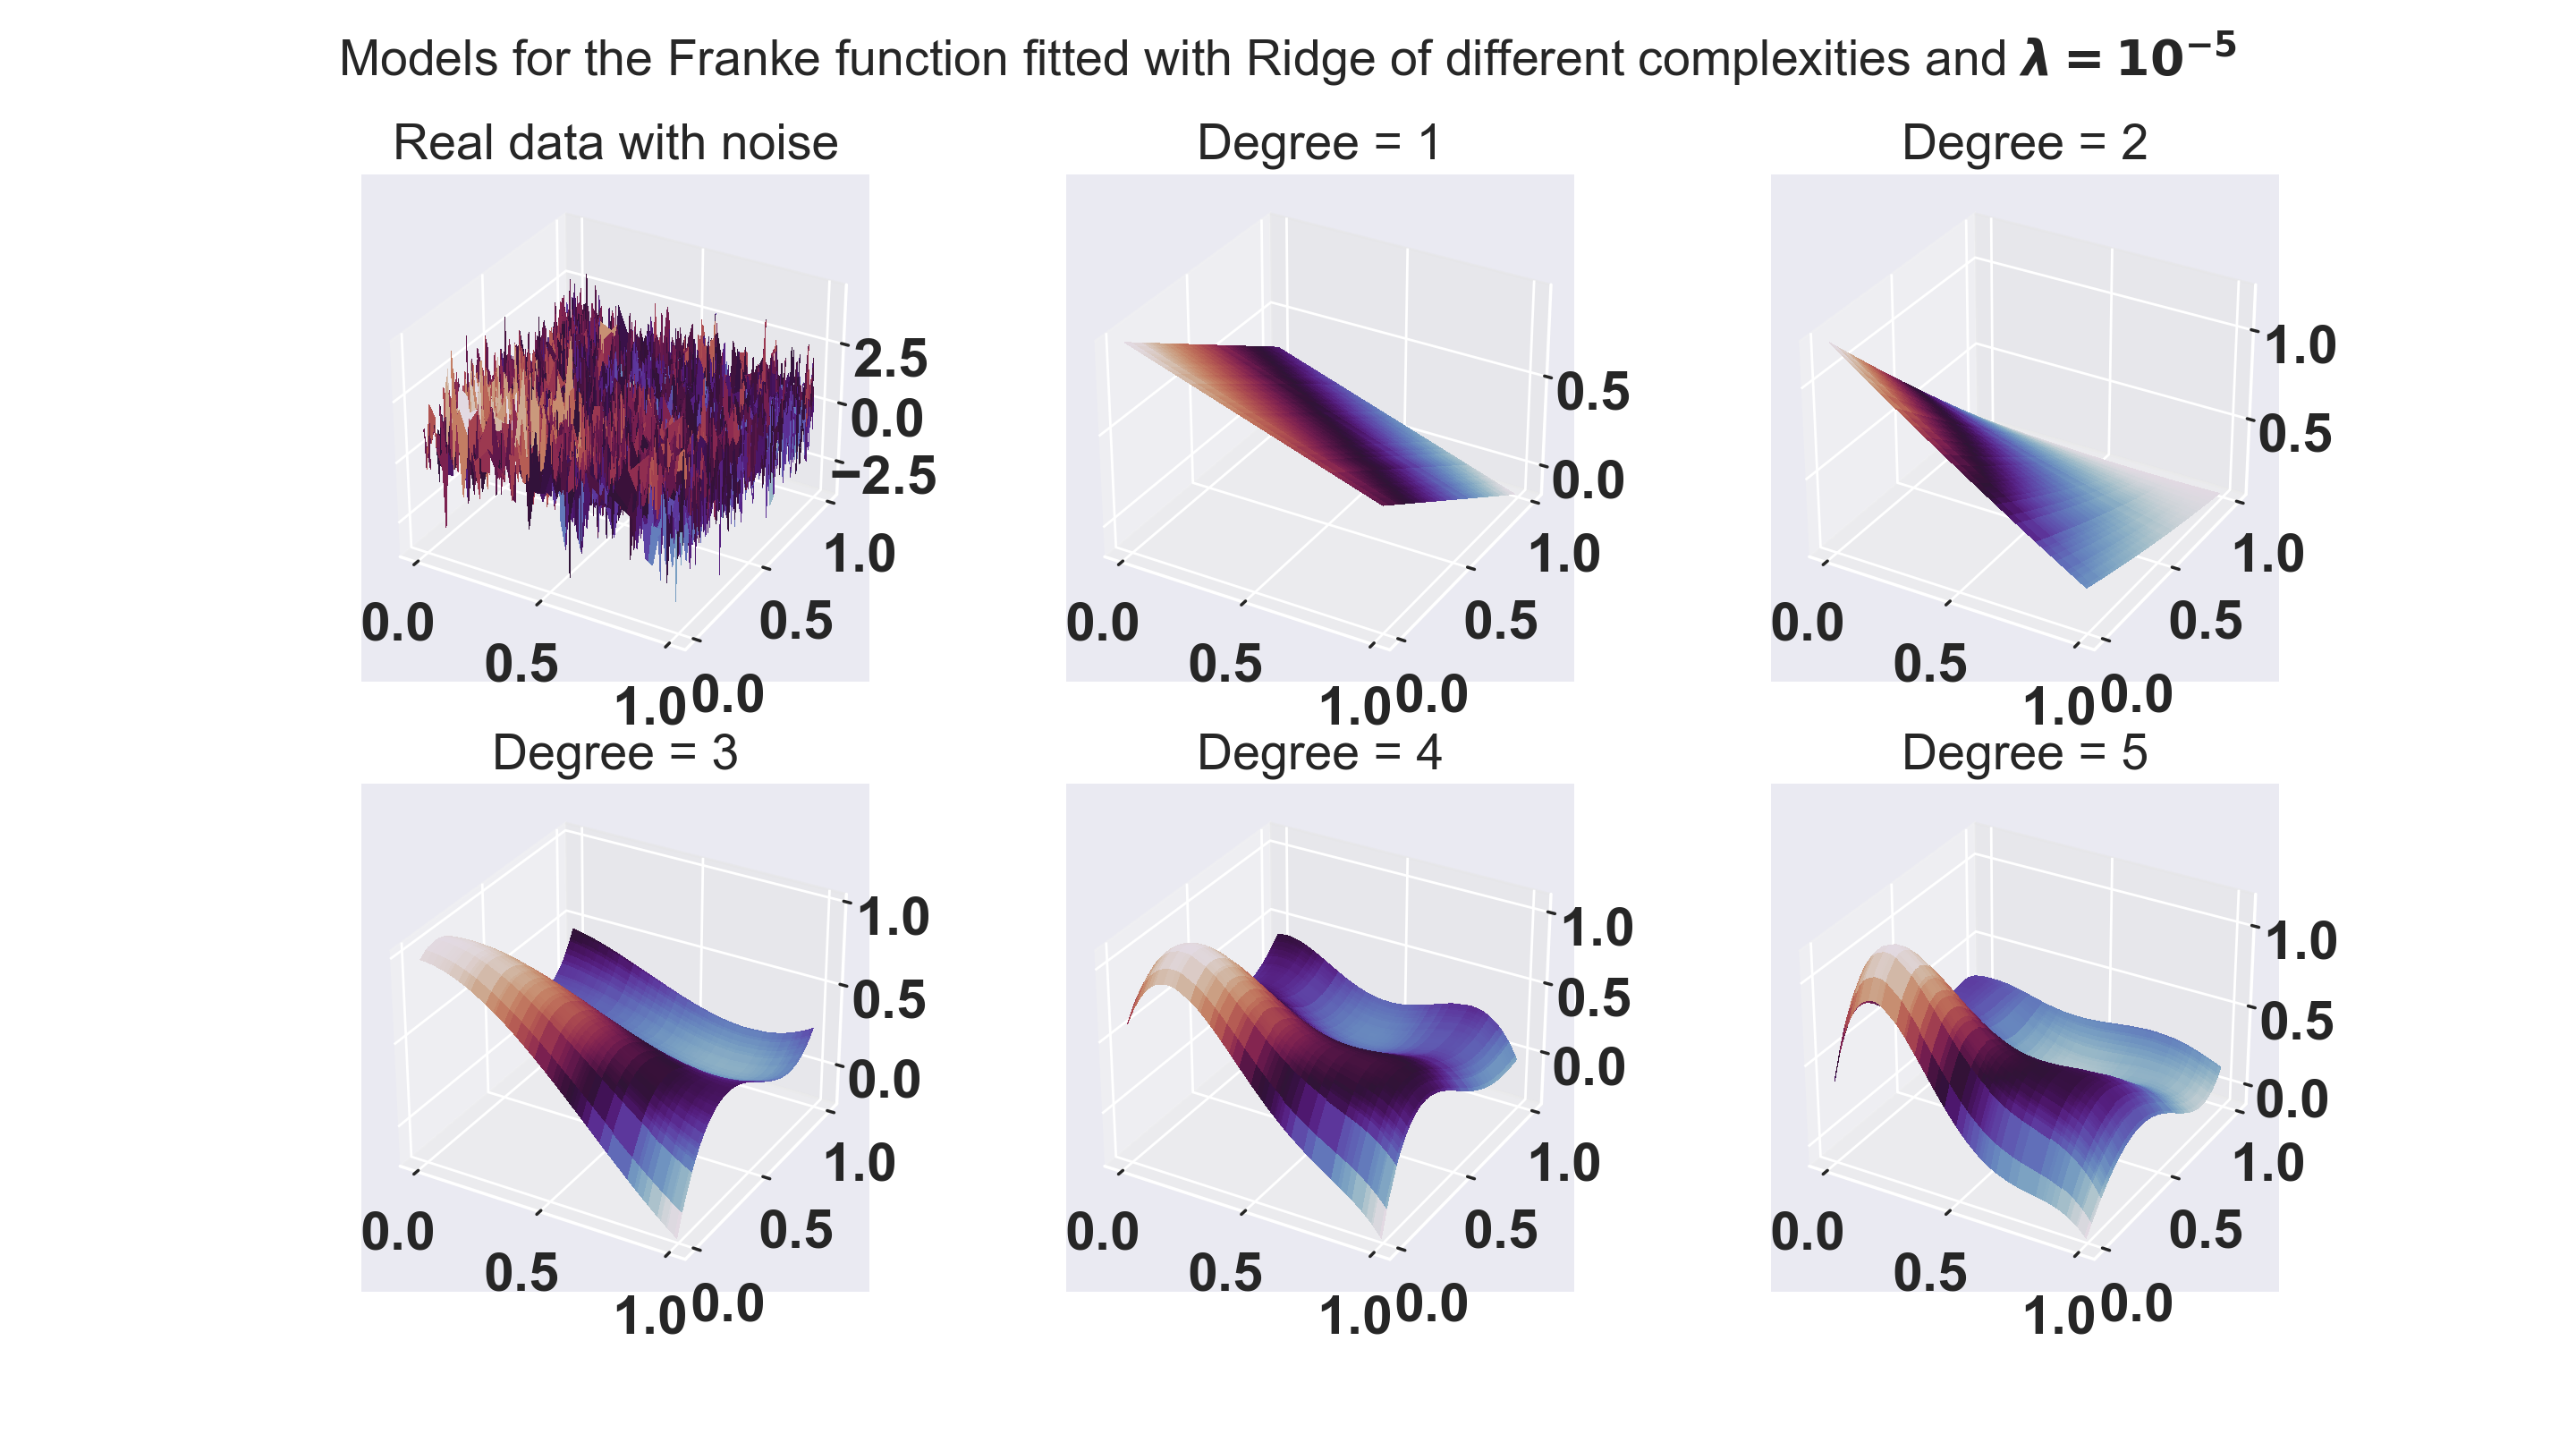
\includegraphics[width=\textwidth]{Figure_6.png}
	\caption{}
	\label{Ridge figure}
\end{figure*}

\begin{figure*}[h]
	\centering
	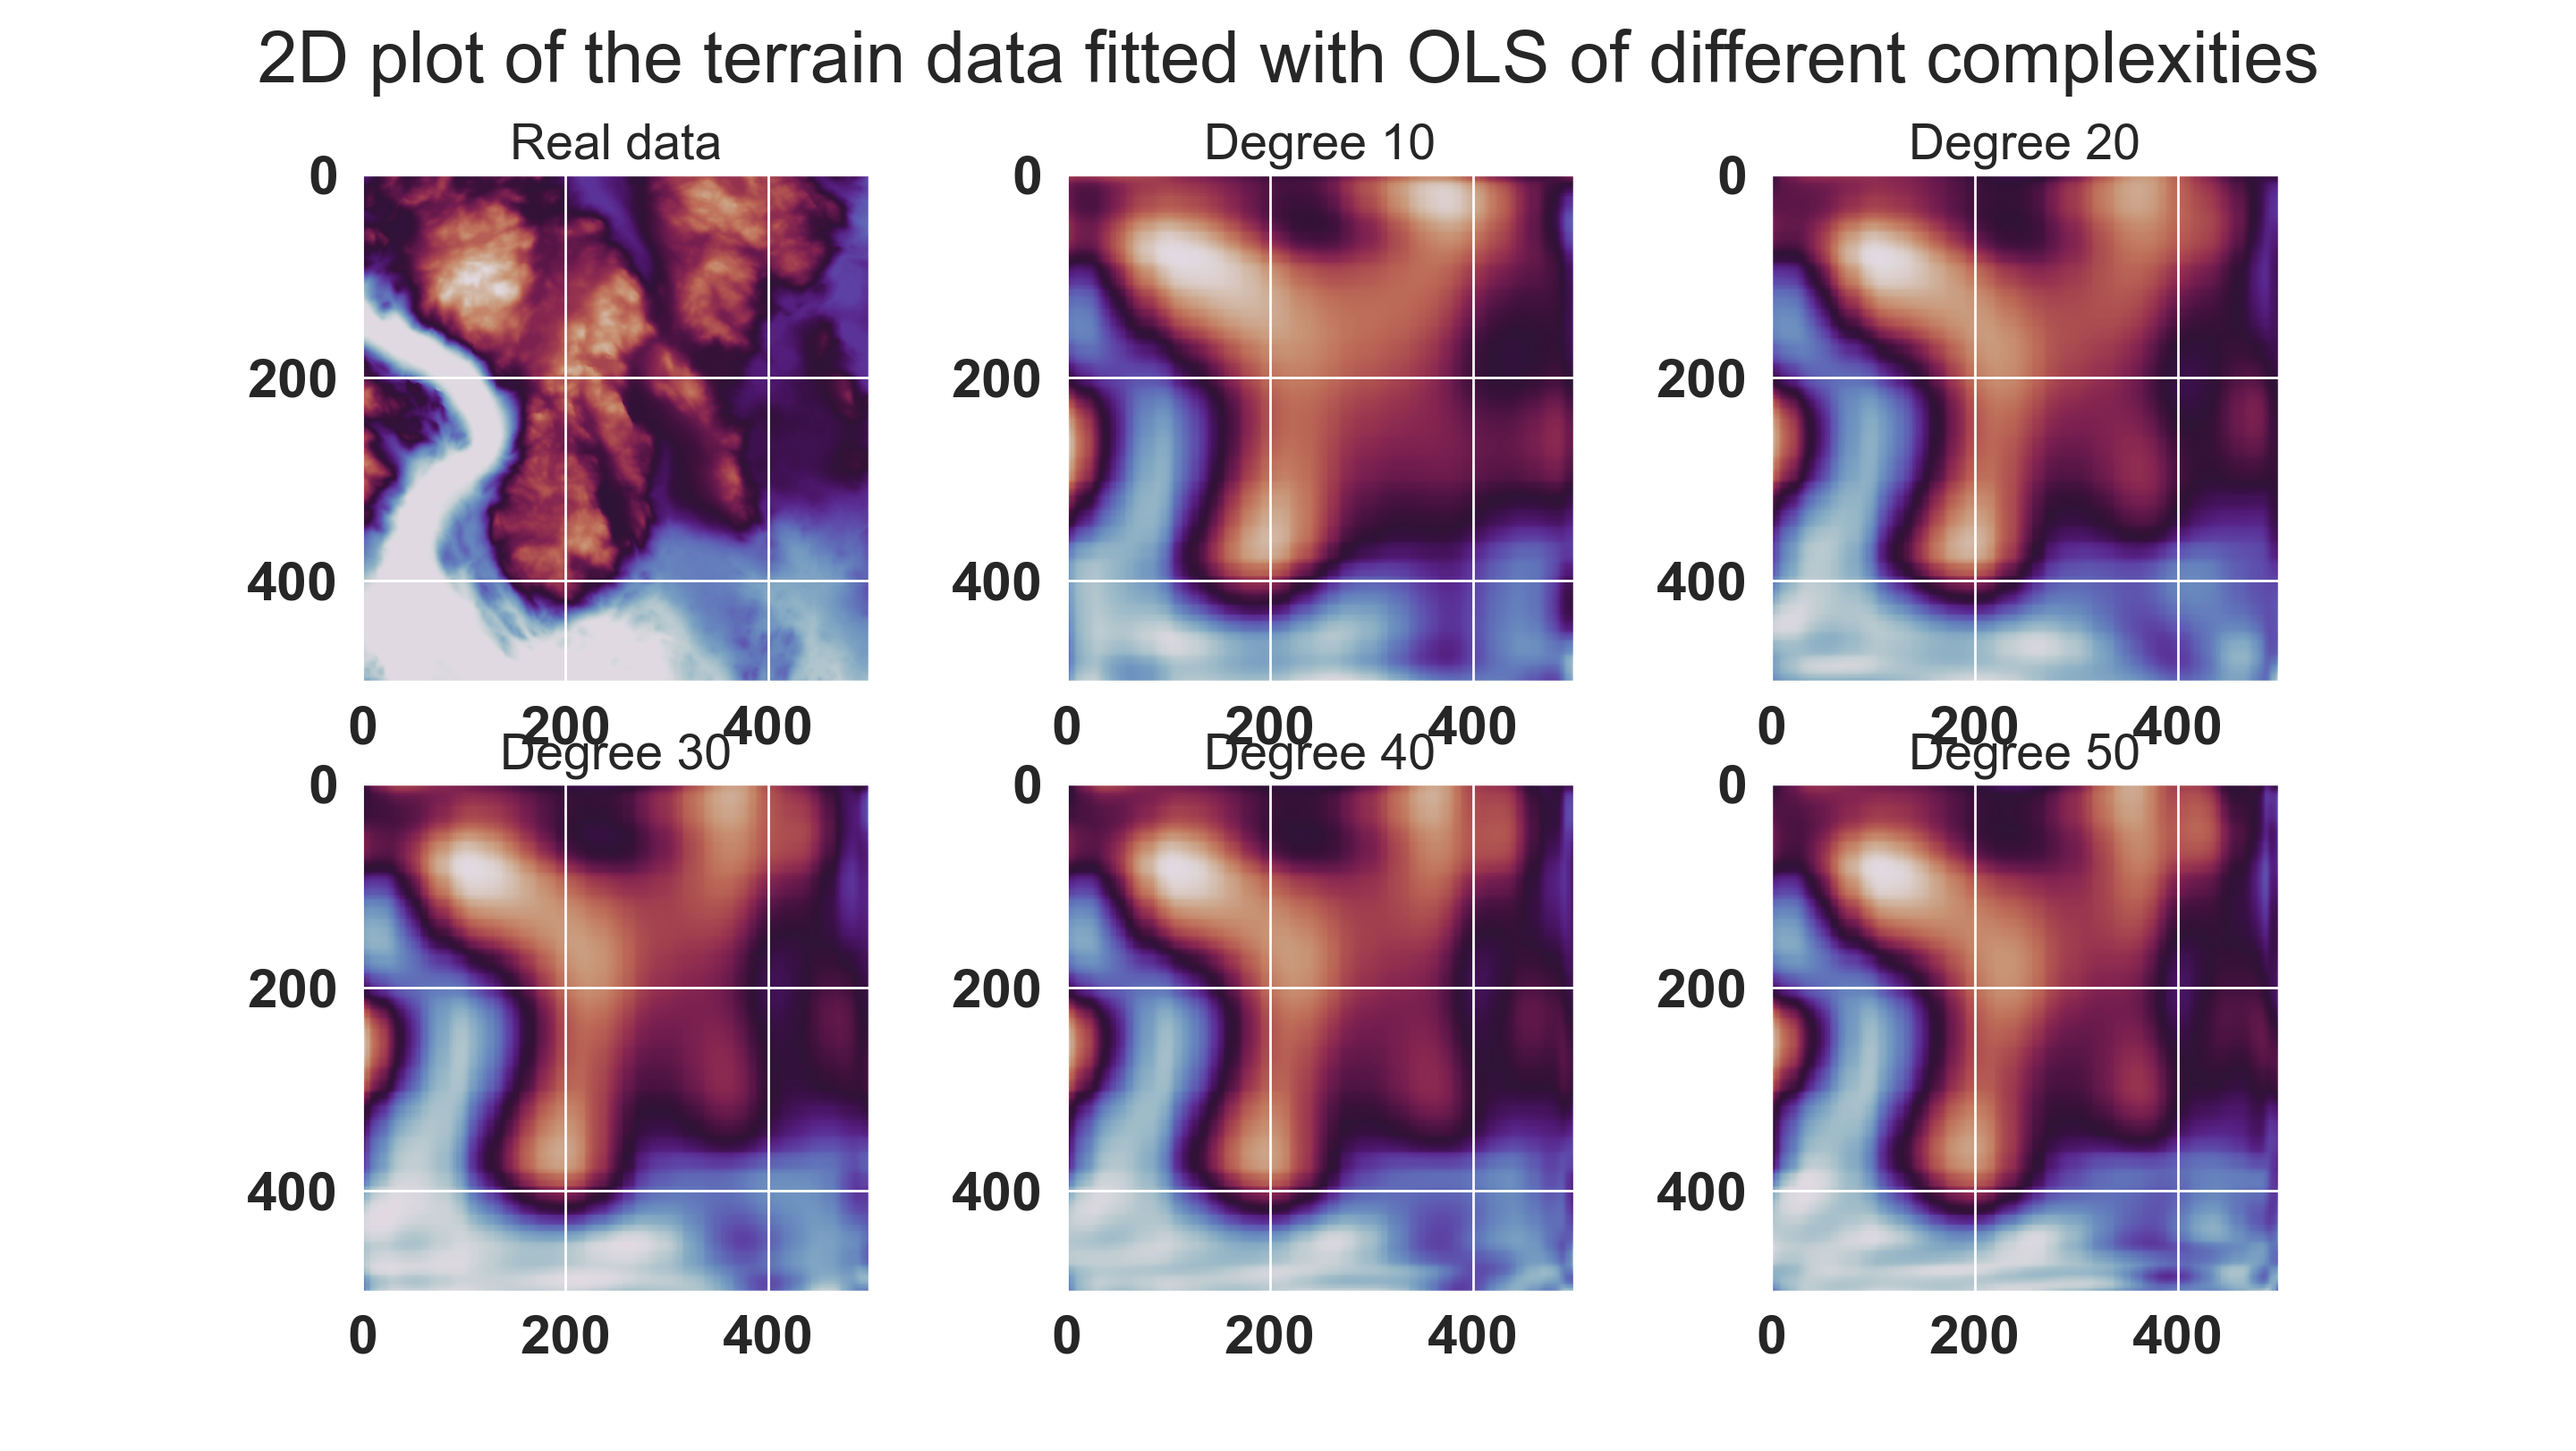
\includegraphics[width=\textwidth]{Figure_5.png}
	\caption{}
	\label{OLS figure terrain data}
\end{figure*}
\subsection{Results for terrain data}

\section{Discussion}
\thispagestyle{plain}

\noindent From figure \eqref{MSE and R2 OLS} we see that when our data set does not include noise
the MSE for the training data gets lower with increas in complexity, while 
the R2 score gets closer and closer to 1. But when we introduce noise whe see from figure \eqref{MSE and R2 OLS noise}
that for our test data the MSE acctually increase with higher complexity. 

The dataset containing the test data consists of $20\%$ of the original
dataset. This implies that the number of points in the test data is 
significantly smaller than that in the training data. We anticipate 
that by increasing the number of data points, the MSE for the model 
created using the test data will converge towards that of the training
model.
\section{Conclusion}
\thispagestyle{plain}
\noindent To summarize our findings, it is clear that the choice of the best regression method depends on the data set used. In scenarios where the data is noise-free, OLS proves to be the most effective regression method. But noise-free data is usually not the case. What we found was that the best regression method for the Franke function with noise given by the normal distribution $\mathcal{N}(0, 0.1)$, was Ridge for higher polynomial degrees, this is due to OLS over-fitting the data to the noise for higher polynomial degrees, while Ridge and LASSO tries to minimise the variance in $\beta$ values to avoid this problem. 
Even though LASSO aims to minimize variance in $\beta$ values, it exhibited the worst performance among the three regression methods. However, it remains uncertain whether Lasso could outperform Ridge and OLS in handling noise due to limitations in iterations. The decision to restrict iterations was influenced by run time constraints, leaving the true capabilities of Lasso in this scenario unknown.
\noindent For our terrain data we surprisingly found that OLS gave the model with the lowest MSE. From what we can see in figure \eqref{OLS 3D figure terrain data} the terrain data looks a little noise, but it may be due to the scaling of the data set that makes OLS the best regression method for the terrain data. 

\noindent The improvement potential for this project is high, due to some grope problems we got started on the project late together as one group. Therefor the structure on GitHub and the cods are quite messy. This is something we will work on improving for the next project. 
% acknowledgements (optional)



%% When it comes to the bibliography I personally generate it using BibLaTeX. (see the link above if you're interested)
%% You're obviously allowed to create the references section however you like.
%% I'll keep it simple here.
\section*{References}  % the asterisk (*) after \section makes the section numbering go away
\bibliographystyle{plain}
\bibliography{citation} 
\newpage
%% if you want to include an appendix, this is how you do it
\clearpage
\onecolumngrid
\appendix
\pagenumbering{alph}

\thispagestyle{plain}

We have assumed that our data can be described by the continous function 
$f(\boldsymbol{x})$, and an error term $\boldsymbol{\epsilon} ~ N(0, \sigma^{2})$. 
If we approximate the function with the solution derived from a model $\boldsymbol{\tilde{y}} = X\boldsymbol{\beta}$ the data can be described with $\boldsymbol{y} = X\boldsymbol{\beta} + \boldsymbol{\epsilon}$. 
The expectation value 

\begin{align*}
    %\hskip\parindent
    \mathbb{E}(\boldsymbol{y}) &= \mathbb{E}(X\boldsymbol{\beta} + \boldsymbol{\epsilon}) \\
    &= \mathbb{E}(X\boldsymbol{\beta}) + \mathbb{E}(\boldsymbol{\epsilon}) && \text{where the expected value $\boldsymbol{\epsilon} = 0$} \\
    \mathbb{E}(y_{i}) &= \sum_{j=0}^{P-1} X_{i,j} \beta_{j} && \text{for the each element} \\
    &= X_{i,*} \beta_{i} && \text{where $_{*}$ replace the sum over index $i$} \\
\end{align*}


The variance for the element $y_{i}$ can be found by
\begin{align*}
    \mathbb{V}(y_{i}) &= \mathbb{E} \big[ (y_{i} - \mathbb{E}(y_{i}))^{2} \big] \\
    &= \mathbb{E} (y_{i}^{2}) - (\mathbb{E}(y_{i})^{2}) \\
    &= \mathbb{E} ((X_{i,*} \beta_{i} + \epsilon_{i})^{2}) - (X_{i,*} \beta_{i})^{2} \\
    &= \mathbb{E} ((X_{i,*} \beta_{i})^{2} + 2\epsilon_{i}X_{i,*} \beta_{i} + \epsilon^{2}) - (X_{i,*} \beta_{i})^{2} \\
    &= \mathbb{E} ((X_{i,*} \beta_{i})^{2}) + \mathbb{E} (2\epsilon_{i}X_{i,*} \beta_{i}) + \mathbb{E} (\epsilon^{2}) - (X_{i,*} \beta_{i})^{2} \\
    &= (X_{i,*} \beta_{i})^{2} + \mathbb{E} (\epsilon^{2}) - (X_{i,*} \beta_{i})^{2} \\
    &= \mathbb{E} (\epsilon^{2}) = \sigma^{2} \\
\end{align*}

The expression for the optimal parameter 
\begin{align*}
    \boldsymbol{\hat{\beta}} &= (\boldsymbol{X}^{T} \boldsymbol{X})^{-1} \boldsymbol{X}^{T} \boldsymbol{y} \\
\end{align*}
We find the expected value of $\boldsymbol{\hat{\beta}}$
\begin{align*}
    \mathbb{E}(\boldsymbol{\hat{\beta}}) &= \mathbb{E}((\boldsymbol{X}^{T} \boldsymbol{X})^{-1} \boldsymbol{X}^{T} \boldsymbol{y}) \\
    &= (\boldsymbol{X}^{T} \boldsymbol{X})^{-1} \boldsymbol{X}^{T} \mathbb{E}(\boldsymbol{y}) && \text{using that $\boldsymbol{X}$ is a non-stochastic variable} \\
    &= (\boldsymbol{X}^{T} \boldsymbol{X})^{-1} \boldsymbol{X}^{T} \boldsymbol{X} \boldsymbol{\beta} && \text{using $\mathbb{E}(\boldsymbol{y}) = \boldsymbol{X} \boldsymbol{\beta}$} \\
    &= \boldsymbol{\beta} \\
\end{align*}
we can find the variance by 
\begin{align*}
    \mathbb{V}(\boldsymbol{\hat{\beta}}) &= \mathbb{E} \big[ (\boldsymbol{\hat{\beta}} - \mathbb{E}(\boldsymbol{\hat{\beta}}))^{2} \big] \\
    &= \mathbb{E} (\boldsymbol{\hat{\beta}} \boldsymbol{\hat{\beta}}^{T}) - \mathbb{E}(\boldsymbol{\hat{\beta}})^{2}  \\
    &= \mathbb{E} (((\boldsymbol{X}^{T} \boldsymbol{X})^{-1} \boldsymbol{X}^{T} \boldsymbol{y}) ((\boldsymbol{X}^{T} \boldsymbol{X})^{-1} \boldsymbol{X}^{T} \boldsymbol{y})^{T}) - \boldsymbol{\hat{\beta}}\boldsymbol{\hat{\beta}}^{T}  \\
    &= \mathbb{E} ((\boldsymbol{X}^{T} \boldsymbol{X})^{-1} \boldsymbol{X}^{T} \boldsymbol{y} \boldsymbol{y}^{T} \boldsymbol{X} (\boldsymbol{X}^{T} \boldsymbol{X})^{-1}) - \boldsymbol{\hat{\beta}}\boldsymbol{\hat{\beta}}^{T}  \\
    &= (\boldsymbol{X}^{T} \boldsymbol{X})^{-1} \boldsymbol{X}^{T} \mathbb{E} (\boldsymbol{y} \boldsymbol{y}^{T}) \boldsymbol{X} (\boldsymbol{X}^{T} \boldsymbol{X})^{-1} - \boldsymbol{\hat{\beta}}\boldsymbol{\hat{\beta}}^{T}  \\
    &= (\boldsymbol{X}^{T} \boldsymbol{X})^{-1} \boldsymbol{X}^{T} (\boldsymbol{X} \boldsymbol{\beta} \boldsymbol{\beta}^{T} \boldsymbol{X}^{T} + \sigma^{2}) \boldsymbol{X} (\boldsymbol{X}^{T} \boldsymbol{X})^{-1} - \boldsymbol{\hat{\beta}}\boldsymbol{\hat{\beta}}^{T}  \\
    &= \boldsymbol{\beta} \boldsymbol{\beta}^{T} + \sigma^{2}((\boldsymbol{X}^{T} \boldsymbol{X})^{-1} \boldsymbol{X}^{T} \boldsymbol{X} (\boldsymbol{X}^{T} \boldsymbol{X})^{-1}) - \boldsymbol{\hat{\beta}}\boldsymbol{\hat{\beta}}^{T}  \\
    &= \sigma^{2}(\boldsymbol{X}^{T} \boldsymbol{X})^{-1} \\
\end{align*}

%% If you want to include figure:
%\includegraphics[scale=1.0]{filename}
%% check https://en.wikibooks.org/wiki/LaTeX/Importing_Graphics if you want to know more

\end{document}
